\documentclass[10pt, letterpaper, twocolumn]{article}

%% Language and font encodings
\usepackage[english]{babel}
\usepackage[utf8x]{inputenc}
\usepackage[T1]{fontenc}

% definign page geometry
\usepackage[a4paper, top=2cm, bottom=2cm, left=3cm, right=2cm, marginparwidth=1.75cm]{geometry}
\usepackage{caption, subcaption}
\captionsetup[table]{skip=10pt}
\captionsetup[subfigure]{justification=justified,singlelinecheck=false}

% Useful packages
\usepackage{amsmath, graphicx, multicol, booktabs, float, abstract, placeins, mathtools, chngcntr}
\usepackage[colorinlistoftodos]{todonotes}
\usepackage[colorlinks=true, allcolors=blue]{hyperref}

% section sizing
\usepackage{titlesec}
\titleformat*{\subsection}{\normalsize\bfseries}

% Title
\title{
    \usefont{OT1}{bch}{b}{n}
    \normalfont \normalsize \textsc{STEM Fellowship Big Data Challenge 2020} \\ [10pt]
    \huge Deep learning transcriptomic model for prediction of pan-drug chemotherapeutic sensitivity \\
}
\selectlanguage{english}
\usepackage{authblk}
\author[1]{Eddie Guo}
\author[2]{Mehul Gupta}
\author[1]{Pouria Torabi}
\author[2]{Sunand Kannappan}
\affil[1]{University of Alberta}
\affil[2]{University of Calgary}

% drawing neural network
\usepackage{tikz}
\usetikzlibrary{shapes, arrows}
\tikzset{
  every neuron/.style={
    circle,
    draw,
    minimum size=1cm
  },
  neuron missing/.style={
    draw=none, 
    scale=3,
    text height=0.333cm,
    execute at begin node=\color{black}$\vdots$
  },
}

\usepackage{ifthen}
\newcommand{\foo}[1]{%
  \ifthenelse{\equal{#1}{missing}}
    {}
    {$H^{(1)}_{\l}$}
}

\newcommand{\hehe}[1]{%
  \ifthenelse{\equal{#1}{missing}}
    {}
    {$H^{(2)}_{\l}$}
}

\newcommand{\hehetwo}[1]{%
  \ifthenelse{\equal{#1}{missing}}
    {}
    {$H^{(3)}_{\l}$}
}

\newcommand{\hehethree}[1]{%
  \ifthenelse{\equal{#1}{missing}}
    {}
    {$H^{(4)}_{\l}$}
}

\newcommand{\hehefour}[1]{%
	\ifthenelse{\equal{#1}{missing}}
	{}
	{$H^{(5)}_{\l}$}
}

\newcommand{\lmao}[1]{%
  \ifthenelse{\equal{#1}{missing}}
    {}
    {$I_{\l}$}
}

% define flowchart styles
\tikzstyle{block} = [rectangle, rounded corners, minimum height=3em, draw=black, inner sep=1em]
\tikzstyle[line] = [draw, -latex']
\tikzstyle{stop} = [rectangle, rounded corners, minimum width=2cm, minimum height=0.5cm,text centered, draw=black]
\tikzstyle{arrow} = [thick,->,>=stealth]

\frenchspacing
\setlength{\parskip}{0em}
% to ensure figures are at the top of the page
\makeatletter
	\setlength\@fptop{0\p@}
\makeatother


\begin{document}
% Abstract
\twocolumn[
	\maketitle
	\begin{abstract}
		The emergence of precision oncology approaches has begun to inform clinical decision-making in diagnostic, prognostic, and treatment contexts. High-throughput technology has enabled machine learning algorithms to utilize molecular characteristics of tumours to generate personalized treatments. However, precision oncology studies have yet to generate a predictive biomarker incorporating pan-cancer gene expression profiles to stratify tumours into similar pan-drug sensitivity profiles. Here we show that a neural network with 10 hidden layers accurately classifies pan-cancer cell lines into two distinct chemotherapeutic response groups with respect to a pan-drug dataset with 89.0\% accuracy (AUC = 0.904). Using unsupervised clustering algorithms, we found that a cohort of cell line gene expression data from the Genomics of Drug Sensitivity in Cancer could be clustered into two response groups with significant differences in pan-drug chemotherapeutic sensitivity. After applying the Boruta feature selection algorithm to this dataset, a deep learning model was developed to predict chemotherapeutic response groups. The high classification efficacy of the model validates our postulate that cell lines with similar gene expression profiles present similar pan-drug chemotherapeutic sensitivity, and it provides evidence for the potential utility of similar combinatorial biomarkers for the selection of potent candidate drugs that maximize therapeutic response and minimize cytotoxic burden. Future investigations aim to recursively subcluster within the response clusters defined in this study to provide increasingly granular subsets of patients with similar chemotherapeutic response patterns.
		\vspace{1em}

		% Keywords
		\noindent {\textbf{Keywords}\\
			Clustering, neural network, transcriptomics, chemotherapeutic response, combinatorial biomarker, molecular profile, therapeutic sensitivity, cancer}
	\end{abstract} \vspace{1em}
]

% Introduction
\section{Introduction}
With the advent of high-throughput sequencing technology, precision oncology approaches have utilized molecular characteristics of tumours to inform clinical decision-making, including choice of chemotherapeutic regimen \cite{drugml, patient_resps}. These approaches attempt to improve both targeted and conventional therapeutics. Existing precision oncology approaches have largely focused on the development of targeted therapeutics, which are selective for specific genetic aberrations and expression profiles. Although these approaches may be successful for inducing tumour response, tumours are more likely to gain resistance to therapies with specific targets \cite{small_mol}. Moreover, not all tumours present with targetable features \cite{small_mol}.

Emerging precision oncology approaches have also potentiated the usage of conventional and less targeted chemotherapy. Given that many of these less targeted and consequently more cytotoxic chemotherapies have broad activity, the primary determinants of chemotherapeutic selection include cancer type and certain molecular markers \cite{adverse}. Nevertheless, it is well established that tumour sensitivity to chemotherapy is heterogeneous both between and within cancer types, which results in a subset of patients that fail to respond to conventional chemotherapy regimens while being subjected to significant side effect burden \cite{adjuvant}. Given that evidence suggests that gene expression can mediate drug response, recent advances have utilized individual and combinatorial gene expression biomarkers to develop predictors of tumour sensitivity to chemotherapeutic compounds \cite{integrated}.

While previous studies have developed predictive biomarkers for specific drugs, the utility of these biomarkers is limited to particular patients and clinical contexts \cite{drug_sense}. That is, these studies are limited in terms of clinical generalizability to different chemotherapeutic regimens and cancer types. However, a pan-cancer and pan-drug predictive biomarker may provide significant clinical utility in the selection of candidate therapies for particular patients. Such a biomarker could be developed if tumours with similar expression have similar drug responses across most chemotherapies. The availability of pan-cancer cell line databases with \textit{in vitro} drug sensitivity analyses along with accompanying gene expression profiling provides an ideal model for such analyses \cite{gdsc}. However, the majority of previous drug sensitivity predictive biomarkers built on cell line databases have utilized traditional clinical criteria (ex: tumour location, TP53 and KRAS mutation status), which fail to capture the dimensionality of available transcriptomic data \cite{colorectal,gi,lung,breast}. Furthermore, advanced deep learning approaches that are capable of handling such dimensionality often fail to allow interpretability and consequently require transcriptomic data that is clinically infeasible \cite{ml_oncol}. Thus, deep learning approaches should minimize the number of selected transcriptomic features to maximize both the accuracy and interpretability of such predictive biomarkers in a clinical context. This allows for meaningful pathway functional enrichment analyses which provide a deeper understanding of the underlying biological significance of features contributing to the deep learning model.

In this study, we set out to generate a deep learning transcriptomic model for the prediction of pan-drug chemotherapeutic sensitivity across cell lines of all cancer types. If successful, this would demonstrate that gene expression influences chemotherapeutic response across most drugs and further motivate future studies into the development of clinically applicable predictors of candidate chemotherapeutics for tumours of a specific gene expression profile. Further, this biomarker may prove to be a useful technique to stratify patients into distinct treatment response groups, allowing chemotherapy regimens to be tailored to the transcriptomic characteristics of specific cancers.

Following unsupervised clustering of cell lines into therapeutic response groups with similar pan-drug sensitivity, we show that conventional clinical criteria fail to stratify cell lines by their therapeutic response. This substantiates the existence of substantial chemotherapeutic response heterogeneity between and within these clinical subgroups. Further, this motivates the need for a biomarker capable of accurately classifying tumours into response groups in order to effectively guide clinical management in the context of chemotherapeutic treatment. To create such a predictive marker, we utilize a biologically agnostic feature selection algorithm to identify a subset of 300 relevant genes predictive of chemotherapeutic sensitivity. In this study, we develop a deep learning model from the selected genes, which showcases a strong predictive ability to stratify pan-cancer cell lines into therapeutic response groups.


% Materials and Methods
\section{Methods}
We developed a deep learning model to accurately classify cancer cell lines into therapeutic response groups using data from the Genomics of Drug Sensitivity in Cancer (GDSC) consortium \cite{gdsc}. Following data collection and curation, we utilized unsupervised clustering algorithms to define two groups based on their chemotherapeutic response. Next, we employed a biologically agnostic feature selection algorithm, Boruta, to select statistically relevant genes for our neural network. These transcriptomic features were fed into a neural network that classifies patients into therapeutic response groups as defined by the clustering algorithms. Neural network architectures were optimized using a grid search and evaluated using 5-fold stratified cross-validation on the training data. Final model evaluation was performed on the testing dataset. See Fig. \ref{fig:pipeline} for an overview of the data analysis pipeline.


% flowchart figure
\begin{figure}[!ht]
	\centering
	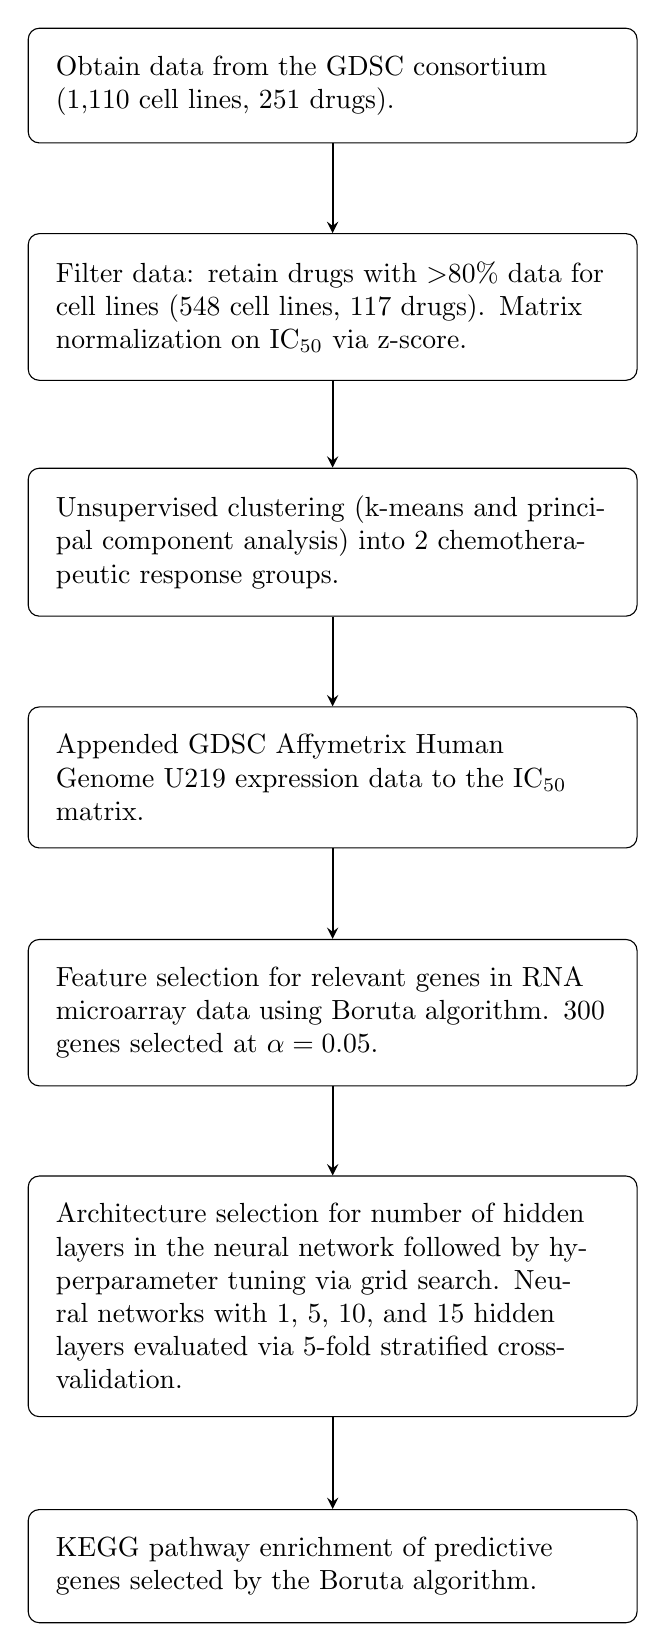
\begin{tikzpicture}[node distance=7em, auto]
	% blocks
	\node [block, text width=20em] (init) {Obtain data from the GDSC consortium (1,110 cell lines, 251 drugs).};
	\node [block, below of=init, text width=20em, yshift=-1em] (process) {Filter data: retain drugs with $>$80\% data for cell lines (548 cell lines, 117 drugs). Matrix normalization on IC$_{50}$ via z-score.};
	\node [block, below of=process, text width=20em, yshift=-1.5em] (kmeans) {Unsupervised clustering (k-means and principal component analysis) into 2 chemotherapeutic response groups.};
	\node [block, below of=kmeans, text width=20em, yshift=-1.5em] (append) {Appended GDSC Affymetrix Human Genome U219 expression data to the IC$_{50}$ matrix.};
	\node [block, below of=append, text width=20em, yshift=-1.5em] (feat) {Feature selection for relevant genes in RNA microarray data using Boruta algorithm. 300 genes selected at $\alpha=0.05$.};
	\node [block, below of=feat, text width=20em, yshift=-3.25em] (neural) {Architecture selection for number of hidden layers in the neural network followed by hyperparameter tuning via grid search. Neural networks with 1, 5, 10, and 15 hidden layers evaluated via 5-fold stratified cross-validation.};
	\node [block, below of=neural, text width=20em, yshift=-2.75em] (annot) {KEGG pathway enrichment of predictive genes selected by the Boruta algorithm.};
	
	% arrows
	\draw [arrow] (init) -- (process);
	\draw [arrow] (process) -- (kmeans);
	\draw [arrow] (kmeans) -- (append);
	\draw [arrow] (append) -- (feat);
	\draw [arrow] (feat) -- (neural);
	\draw [arrow] (neural) -- (annot);
	\end{tikzpicture}
	\caption{Summary of the data analysis pipeline.}
	\label{fig:pipeline}
\end{figure}


\subsection{Determining pan-cancer therapeutic response cohorts}
To better understand the impact and predictive ability of transcriptomic dysregulation in chemotherapeutic response, a pan-cancer cohort of cell lines and associated therapeutic sensitivity data were obtained from the GDSC database. The database includes 1,110 cell lines from various tumour types and is thought to represent a relatively comprehensive pan-cancer dataset. In addition, the acquired dataset contained therapeutic efficacy information in the form of half-maximal inhibitory concentration (IC$_{50}$) values for 251 chemotherapies. These values correspond to the minimal concentration of therapeutic required to induce cell death in 50\% of the cultured cells, with lower values being associated with improved drug efficacy. The dataset was used to generate a matrix with cell lines and accompanying therapeutic information. The matrix was then filtered to exclude therapies with less than 80\% of data for all cell lines, followed by the exclusion of cell lines lacking response data for the drugs retained in the first step. The filtered matrix was analyzed to ensure that it was still representative of a relatively pan-cancer dataset.


\subsection{Identification of pan-cancer therapeutic response cohorts}
Cell line therapeutic sensitivity matrices were used to evaluate whether conventional clinical criteria could separate patients into previously-defined chemotherapeutic response groups. These conventional clinical criteria included anatomic location and solid versus non-solid tumour status, as well as broadly applicable molecular markers -- TP53 and KRAS mutation status \cite{colorectal, gi, lung, breast}. Cell lines were separated into subgroups based on these criteria and visualized to determine whether these criteria effectively clustered response groups.

Following the evaluation of existing classifiers, we attempted to create defined cell line clusters using observed chemotherapeutic response of the pan-cancer cell line samples. We developed a normalized Euclidean distance matrix for the retained cell lines based on their pan-chemotherapy response. The matrix was used to identify the minimum number of clusters capable of representing the therapeutic heterogeneity identified across the cancer cell lines while maintaining significant inter-cluster distance. From the matrix, k-means clustering was utilized to assign cell line candidates to appropriate therapeutic response cohorts (the elbow method was used as a heuristic for determining the number of clusters). Generalized differences in chemotherapeutic efficacy between cohorts were visualized using a heatmap generated by the pheatmap package \cite{pheatmap} in R. The heatmap displayed 2 groups clustered using k-means clustering. The separation between clusters was also visualized using principal component analysis with the plotly package \cite{plotly} in R. Following the identification of defined clusters, differences in therapeutic efficacy between the identified cohorts were evaluated. Mann-Whitney U tests were utilized to compare IC$_{50}$ values between the groups. False discovery rate (FDR) correction was utilized to correct for multiple comparisons. To further validate the existence of these distinct chemotherapeutic response  clusters, intra-cancer heterogeneity was evaluated; 11 cancer subtypes with sufficient cell line representation ($n>20$) were identified. Differences in chemotherapeutic efficacy between cell lines assigned to group A and B were visualized using heatmaps.


% PCA figures
\begin{figure*}[!ht]
	\centering
    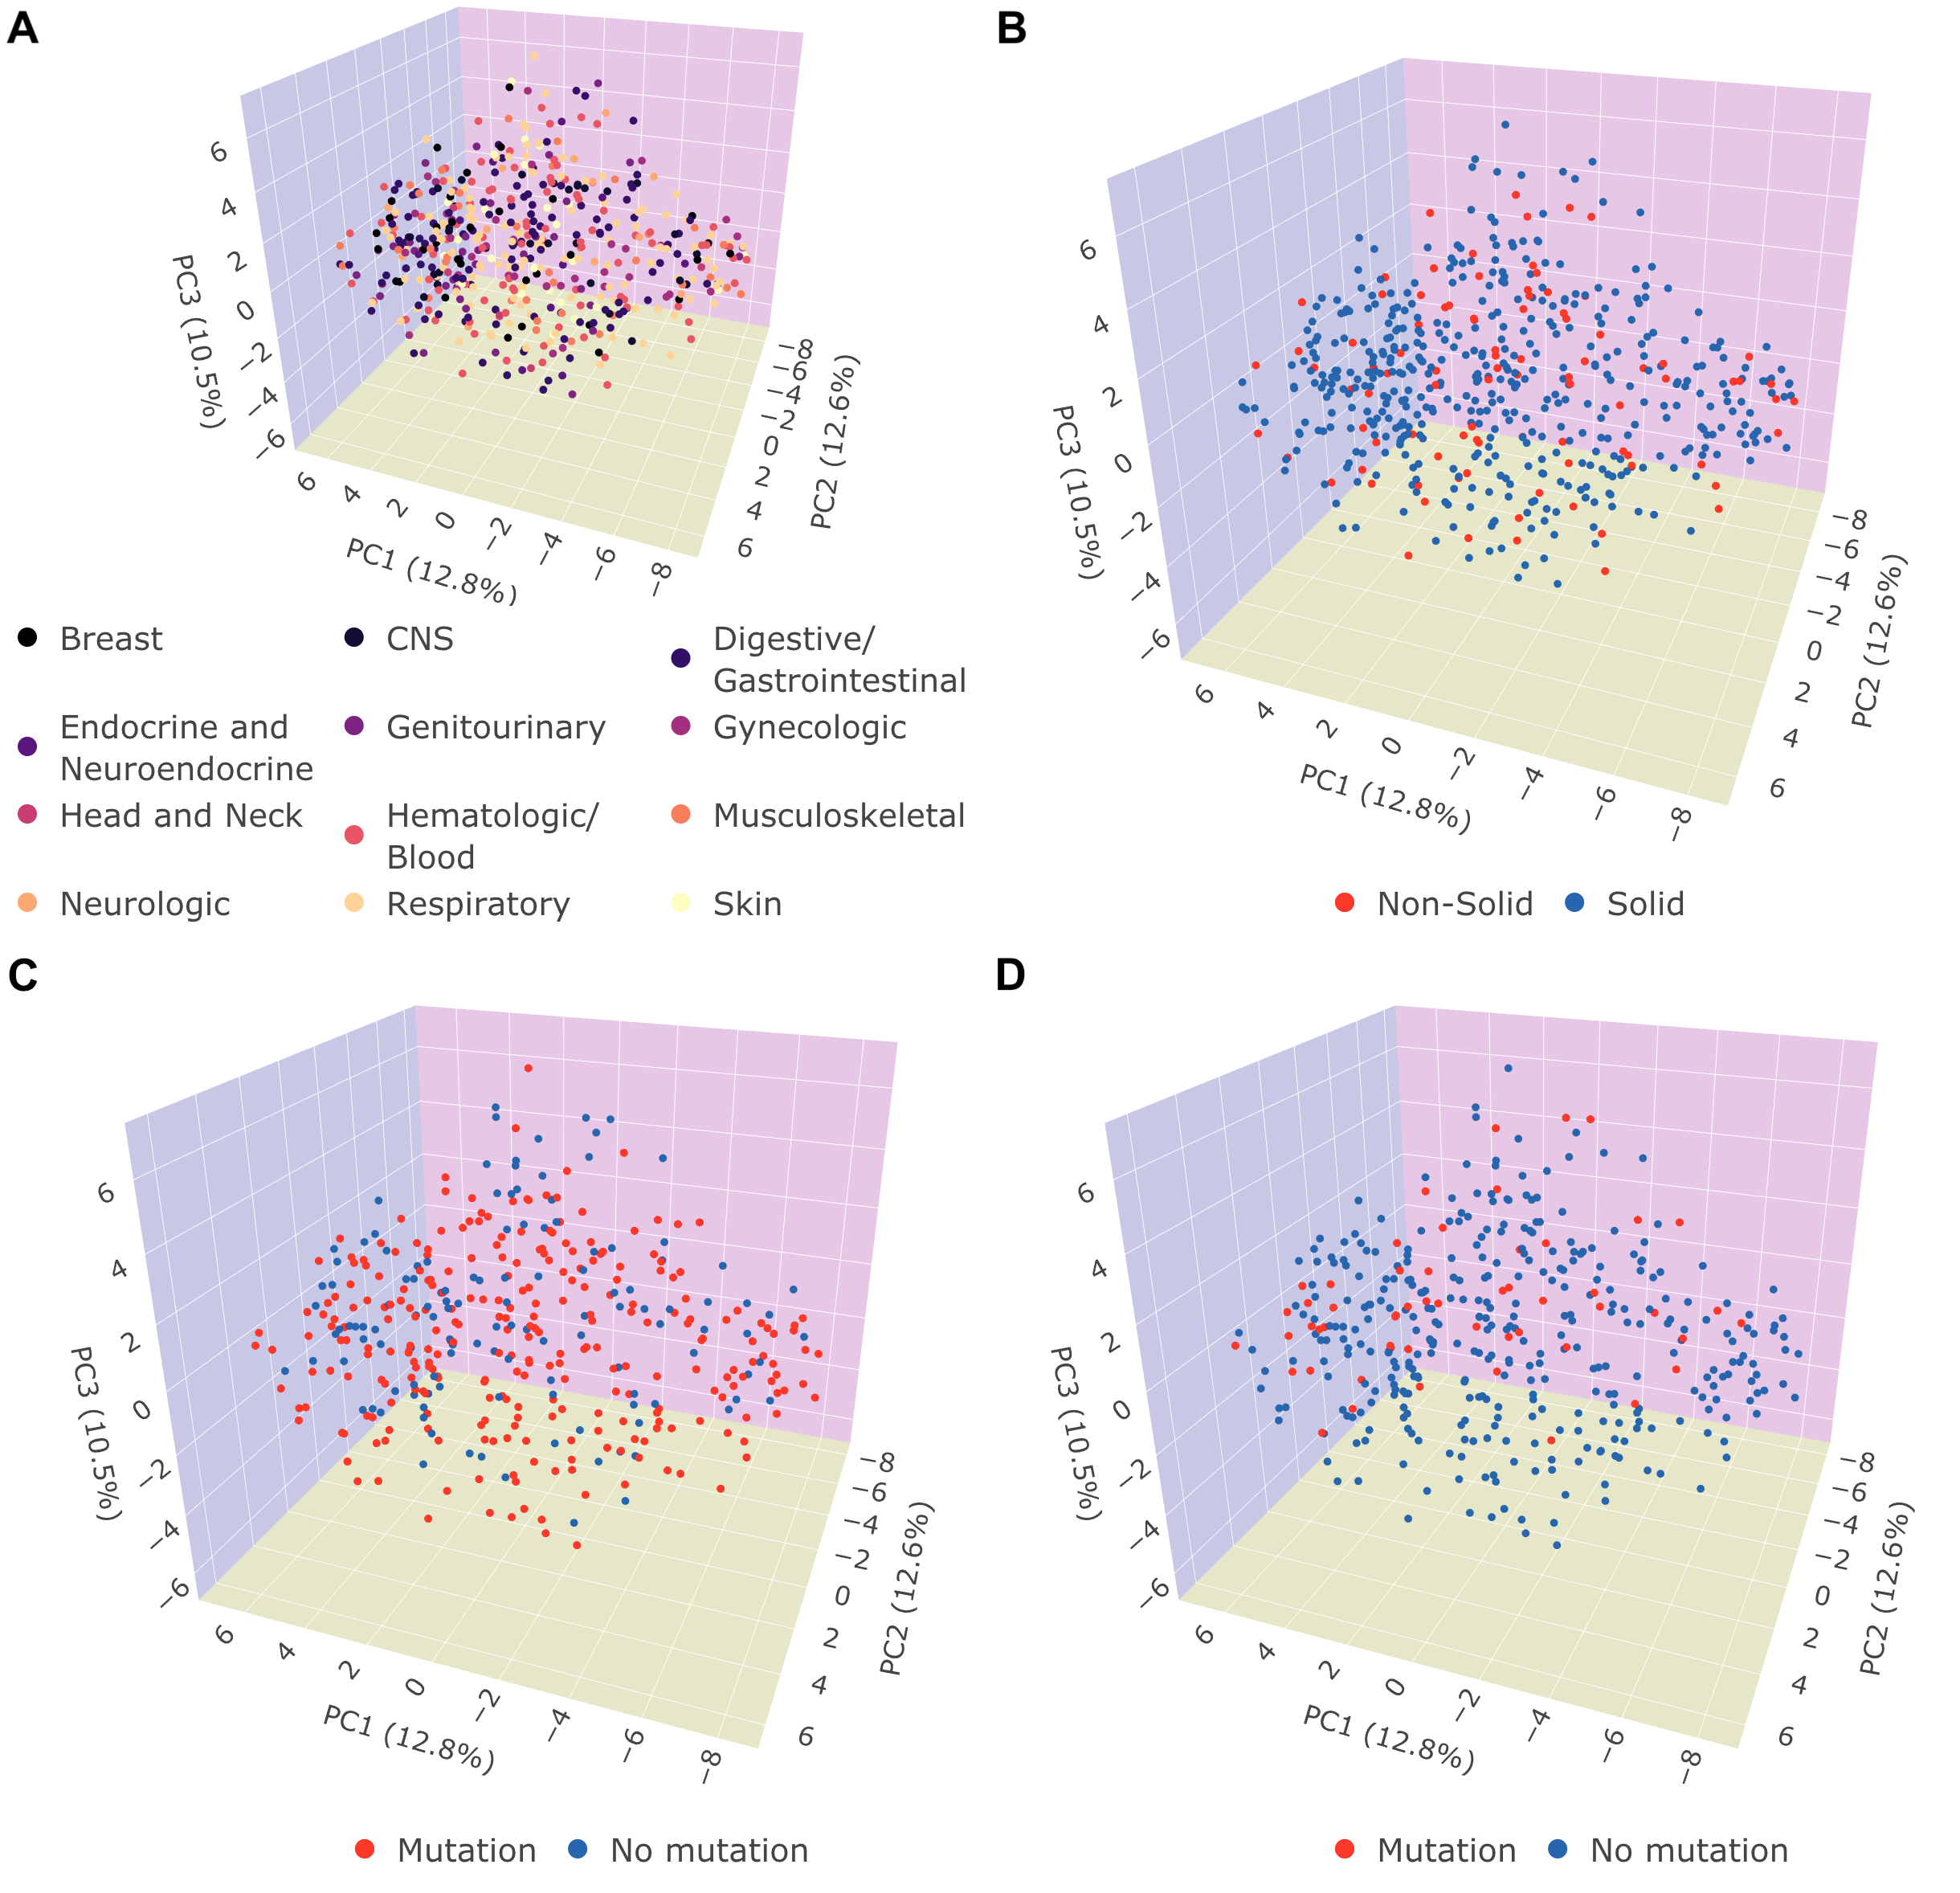
\includegraphics[width=\textwidth]{Figures/initial_pca.png}

	\caption{Principal component analysis of pan-cancer cell line therapeutic efficacy generated from IC$_{50}$ values of all available chemotherapeutics.The x-axis shows the first principal component, the y-axis shows the second component, and the z-axis shows the third principal component. Cell lines are visualized based on major cancer type classifications, including (\textbf{A}) body system of tumour and (\textbf{B}) solid vs. non-solid tumour status. Cell lines were also visualized on major molecular markers, including (\textbf{C}) TP53 mutation status, and (\textbf{D}) KRAS mutation status.}
	\label{fig:overall_pca}
\end{figure*}


% clustering figure
\begin{figure*}[!ht]
    \centering
    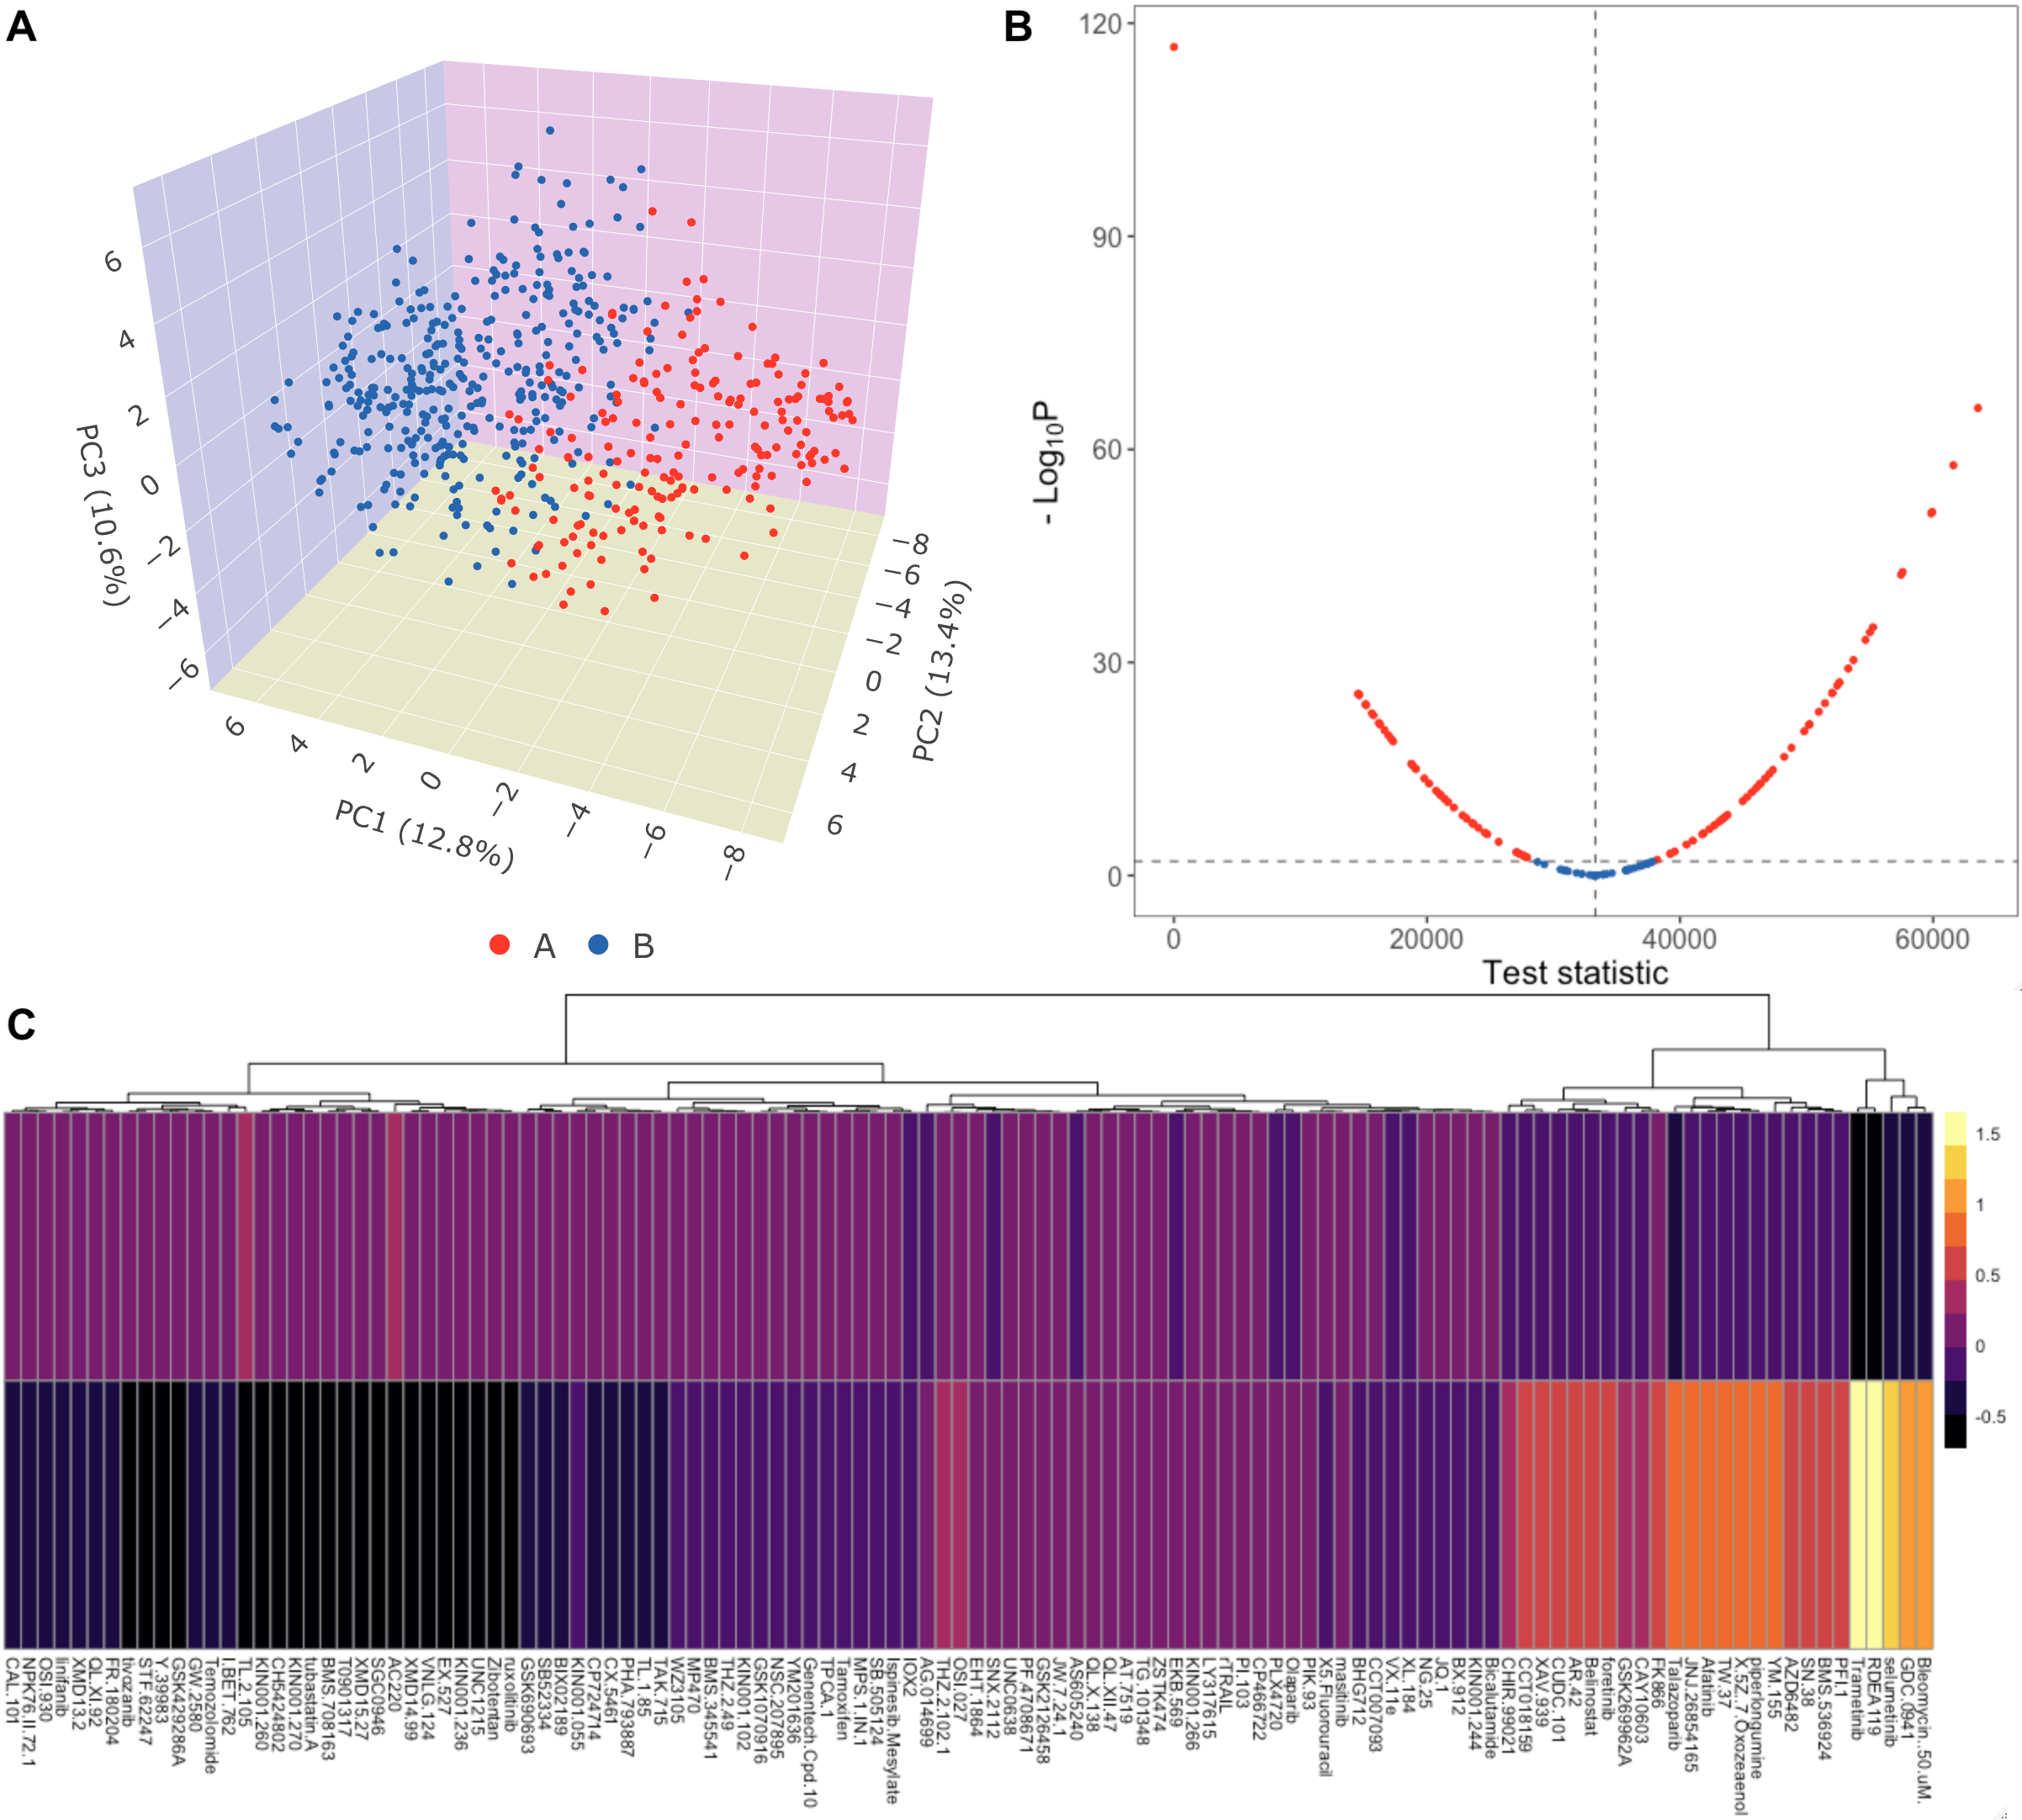
\includegraphics[width=\textwidth]{Figures/clustering.png}

    \caption{(\textbf{A}) Principal component analysis of pan-cancer cell line therapeutic efficacy generated from IC$_{50}$ values of all available chemotherapeutics. The x-axis shows the first principal component, the y-axis shows the second principal component, and the z-axis shows the third principal component. The two identified therapeutic response clusters (A and B) are indicated in red and blue respectively. (\textbf{B}) Volcano plot identifying chemotherapeutics with significantly different IC$_{50}$ values between therapeutic response clusters. Drugs identified in red meet the criteria for significance (FDR adjusted $p<0.05$). (\textbf{C}) Heatmap of therapeutic IC$_{50}$ for the two identified therapeutic response clusters. Columns represent individual chemotherapies and are clustered according to Euclidean distance. Colours range from yellow to black, with a shift toward the latter indicating increased efficacy of the corresponding chemotherapeutic.}
    \label{fig:clustering}
\end{figure*}


\subsection{Feature Selection with Boruta}
In order to develop a transcriptomic model predictive of therapeutic response clusters, we retrieved expression data quantified by the GDSC consortium using the Affymetrix U219 microarray for each candidate cell line. Here, minimally processed CEL files were obtained from ArrayExpress (ascension number E-MTAB-3610) and processed using the affy package \cite{affy} in R. The resulting normalized expression matrix for candidate cell lines was then merged with the existing dataset. This addition resulted in the loss of 7 cell lines (2 from cluster A and 5 from cluster B), resulting in the inclusion of 541 cell lines in model generation. The microarray dataset quantified the expression of 16,382 genes; a model developed from a feature space this large is likely to exhibit high multicollinearity and subsequently overfit, compromising the generalizability of the model. In addition, the large feature space limits the efficiency of various feature selection algorithms (for example, univariate selection or recursive feature elimination), as well as training and optimizing neural networks. We addressed these issues with the Boruta feature selection algorithm using the BorutaPy package \cite{liu} in Python 3. Boruta is a feature selection algorithm based on Random Forest classification which iteratively removes features that are statistically less significant than a shuffled version of the same feature \cite{kursa}. To better understand the transcriptomic heterogeneity underlying the therapeutic response cohorts, a KEGG pathway enrichment analysis was performed on feature-selected genes used in the deep learning model.


\subsection{Classification of cell lines using an optimized neural network}
The neural network was constructed using the Tensorflow Keras sequential deep learning API \cite{keras} in Python 3. The model underwent multiple instances of optimization, beginning with the depth of the network (1, 5, 10, and 15 hidden layers were evaluated). The rectified linear unit (ReLu) was chosen as the neuronal activation function for input and hidden layers. The output layer used a sigmoid activation for binary classification of inputs (i.e., chemotherapeutic response groups). The neural network was carefully monitored for overfitting on the training dataset. To minimize overfitting, we applied L2 kernel regularization ($\lambda=10^{-3}$), batch normalization, and dropout layers with a 0.3 dropout rate to each hidden layer.

The dataset was randomly segregated using the Pareto principle \cite{pareto}; we reserved 80\% of the data (432 training samples, 541 total) for training and the remaining 20\% for testing. Model selection was performed by hyperparameter tuning using a grid search followed by 5-fold stratified cross-validation on the training data (Table \ref{tab:params}). All grid searches were performed with 3-fold cross-validation on the training data to determine the parameters that minimize the binary cross-entropy loss function. GridSearchCV from the scikit-learn library \cite{scikit-learn} was used to iterate through combinations of epochs, batch size, neurons per hidden layer, L2 regularization penalty, optimizer, and kernel initializer to find the optimal model (Table \ref{tab:params}). To prevent class imbalance during training, we used the Synthetic Minority Oversampling Technique (SMOTE) from the imblearn package \cite{imblearn} for Python 3 to generate synthetic data on the training and validation datasets only. Each model’s performance on the validation dataset was evaluated by the Area Under Curve (AUC) value of the receiver operating characteristic (ROC) curve.

Following grid search and cross-validation, we evaluated the performance of our model on the testing data. Youden's index from the ROC curves corresponding to each neural network’s performance on the training dataset was used to determine the optimal threshold to classify cell lines into chemotherapeutic response groups for the testing dataset. Youden’s index ranges from 0 to 1 inclusive, and an index of 0 indicates that the binary classifier is no better than that obtained from a fair coin flip. Conversely, a value of 1 indicates that the test is perfect (i.e., no false positives or false negatives). The formula for Youden's index is defined as $$J \doteq \text{sensitivity} + \text{specificity} - 1$$ All indices were obtained from the ROC curves by an iterative search for the maximum $J$. That is, $$J = \text{argmax(TPR} - \text{FPR)}$$ where TPR and FPR ($\text{FPR} = 1 - \text{specificity}$) are arrays containing the true positive and false positive rate corresponding to each point on the ROC curve. The threshold corresponding to $J$ was used to classify cell lines. The neural network performance on the testing dataset was visualized using ROC curves and confusion matrices.


% Results
\section{Results}
\subsection{Clustering of pan-cancer cell lines identifies two distinct therapeutic response cohorts}
From the GDSC consortium, we included 548 cell lines (49.4\% of the original cell lines) and 117 (46.6\% of the original drugs) chemotherapeutics for response group clustering. Further analysis of the filtered dataset suggested that it was still representative of a pan-cancer dataset. Next, we assessed the ability of common molecular and clinical characteristics using principal component analysis (PCA) to stratify cell lines into groups with similar chemotherapeutic performance by subgrouping cell lines based upon these criteria. It is clear that common molecular markers such as TP53 and  KRAS mutation status, as well as clinical markers like cancer type or solidity are unable to effectively stratify chemotherapeutic efficacy (Fig. \ref{fig:overall_pca}).

To identify defined cohorts of pan-cancer cell lines with similar trends in therapeutic sensitivity, we employed unsupervised clustering of retained cell lines. PCA was used to reduce the dimensionality of the normalized dataset, allowing for visualization of defined therapeutic response groups. This process identified two distinct clusters of therapeutic sensitivity (Fig. \ref{fig:clustering}), 362 cell lines identified in response group A, and 186 cell lines identified in response group B. That is, the cohorts perform substantially differently in a variety of therapeutics (Fig. \ref{fig:clustering}). To quantify differences in the therapeutic response between these clusters, IC$_{50}$ values were compared between candidate cell lines (Fig. \ref{fig:clustering}). Of the 117 therapies included, 95 had significant differences in efficacy between the identified cohorts, suggesting that each represents groups of cell lines with vastly different therapeutic responses. Comparison of identified chemotherapeutic response cohorts between cancer subtypes shows considerable intra-cancer chemotherapeutic heterogeneity (Fig. \ref{fig:intra}).


\subsection{Boruta selects 300 genes from the 16,382 gene dataset}
The Boruta algorithm was used to select genes that are estimated to have the greatest predictive contribution. The feature selection algorithm identified 300 relevant genes from the original set of 16,382 genes at $\alpha=0.05$ with a maximum tree depth of 5. KEGG pathway functional enrichment performed on the selected genes identified gene sets associated with focal adhesion and PI3K signalling pathways among others (Fig. \ref{fig:kegg}).


% gene annotation figure
\begin{figure}[t]
	\centering
	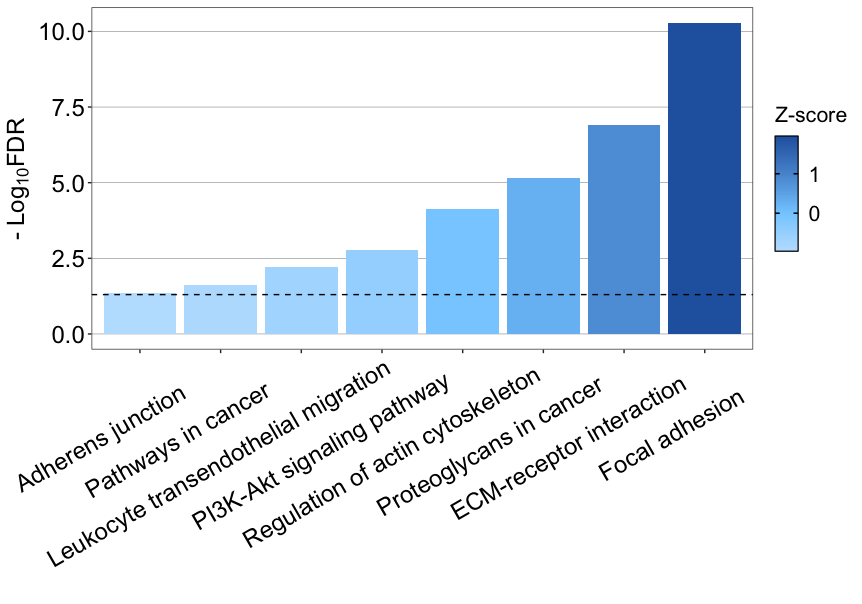
\includegraphics[width=\columnwidth]{Figures/kegg.png}
	\caption{KEGG pathway functional enrichment for feature-selected genes included in the deep learning model. The vertical dotted line indicates the threshold for significance (adjusted $p < 0.05$).}
	\label{fig:kegg}
\end{figure}


\subsection{A neural network with 10 hidden layers accurately classifies patients into responder and non-responder cohorts}


% neural net evaluation figure
\begin{figure*}[!ht]
	\centering
	\begin{subfigure}[t]{\textwidth}
		\centering
		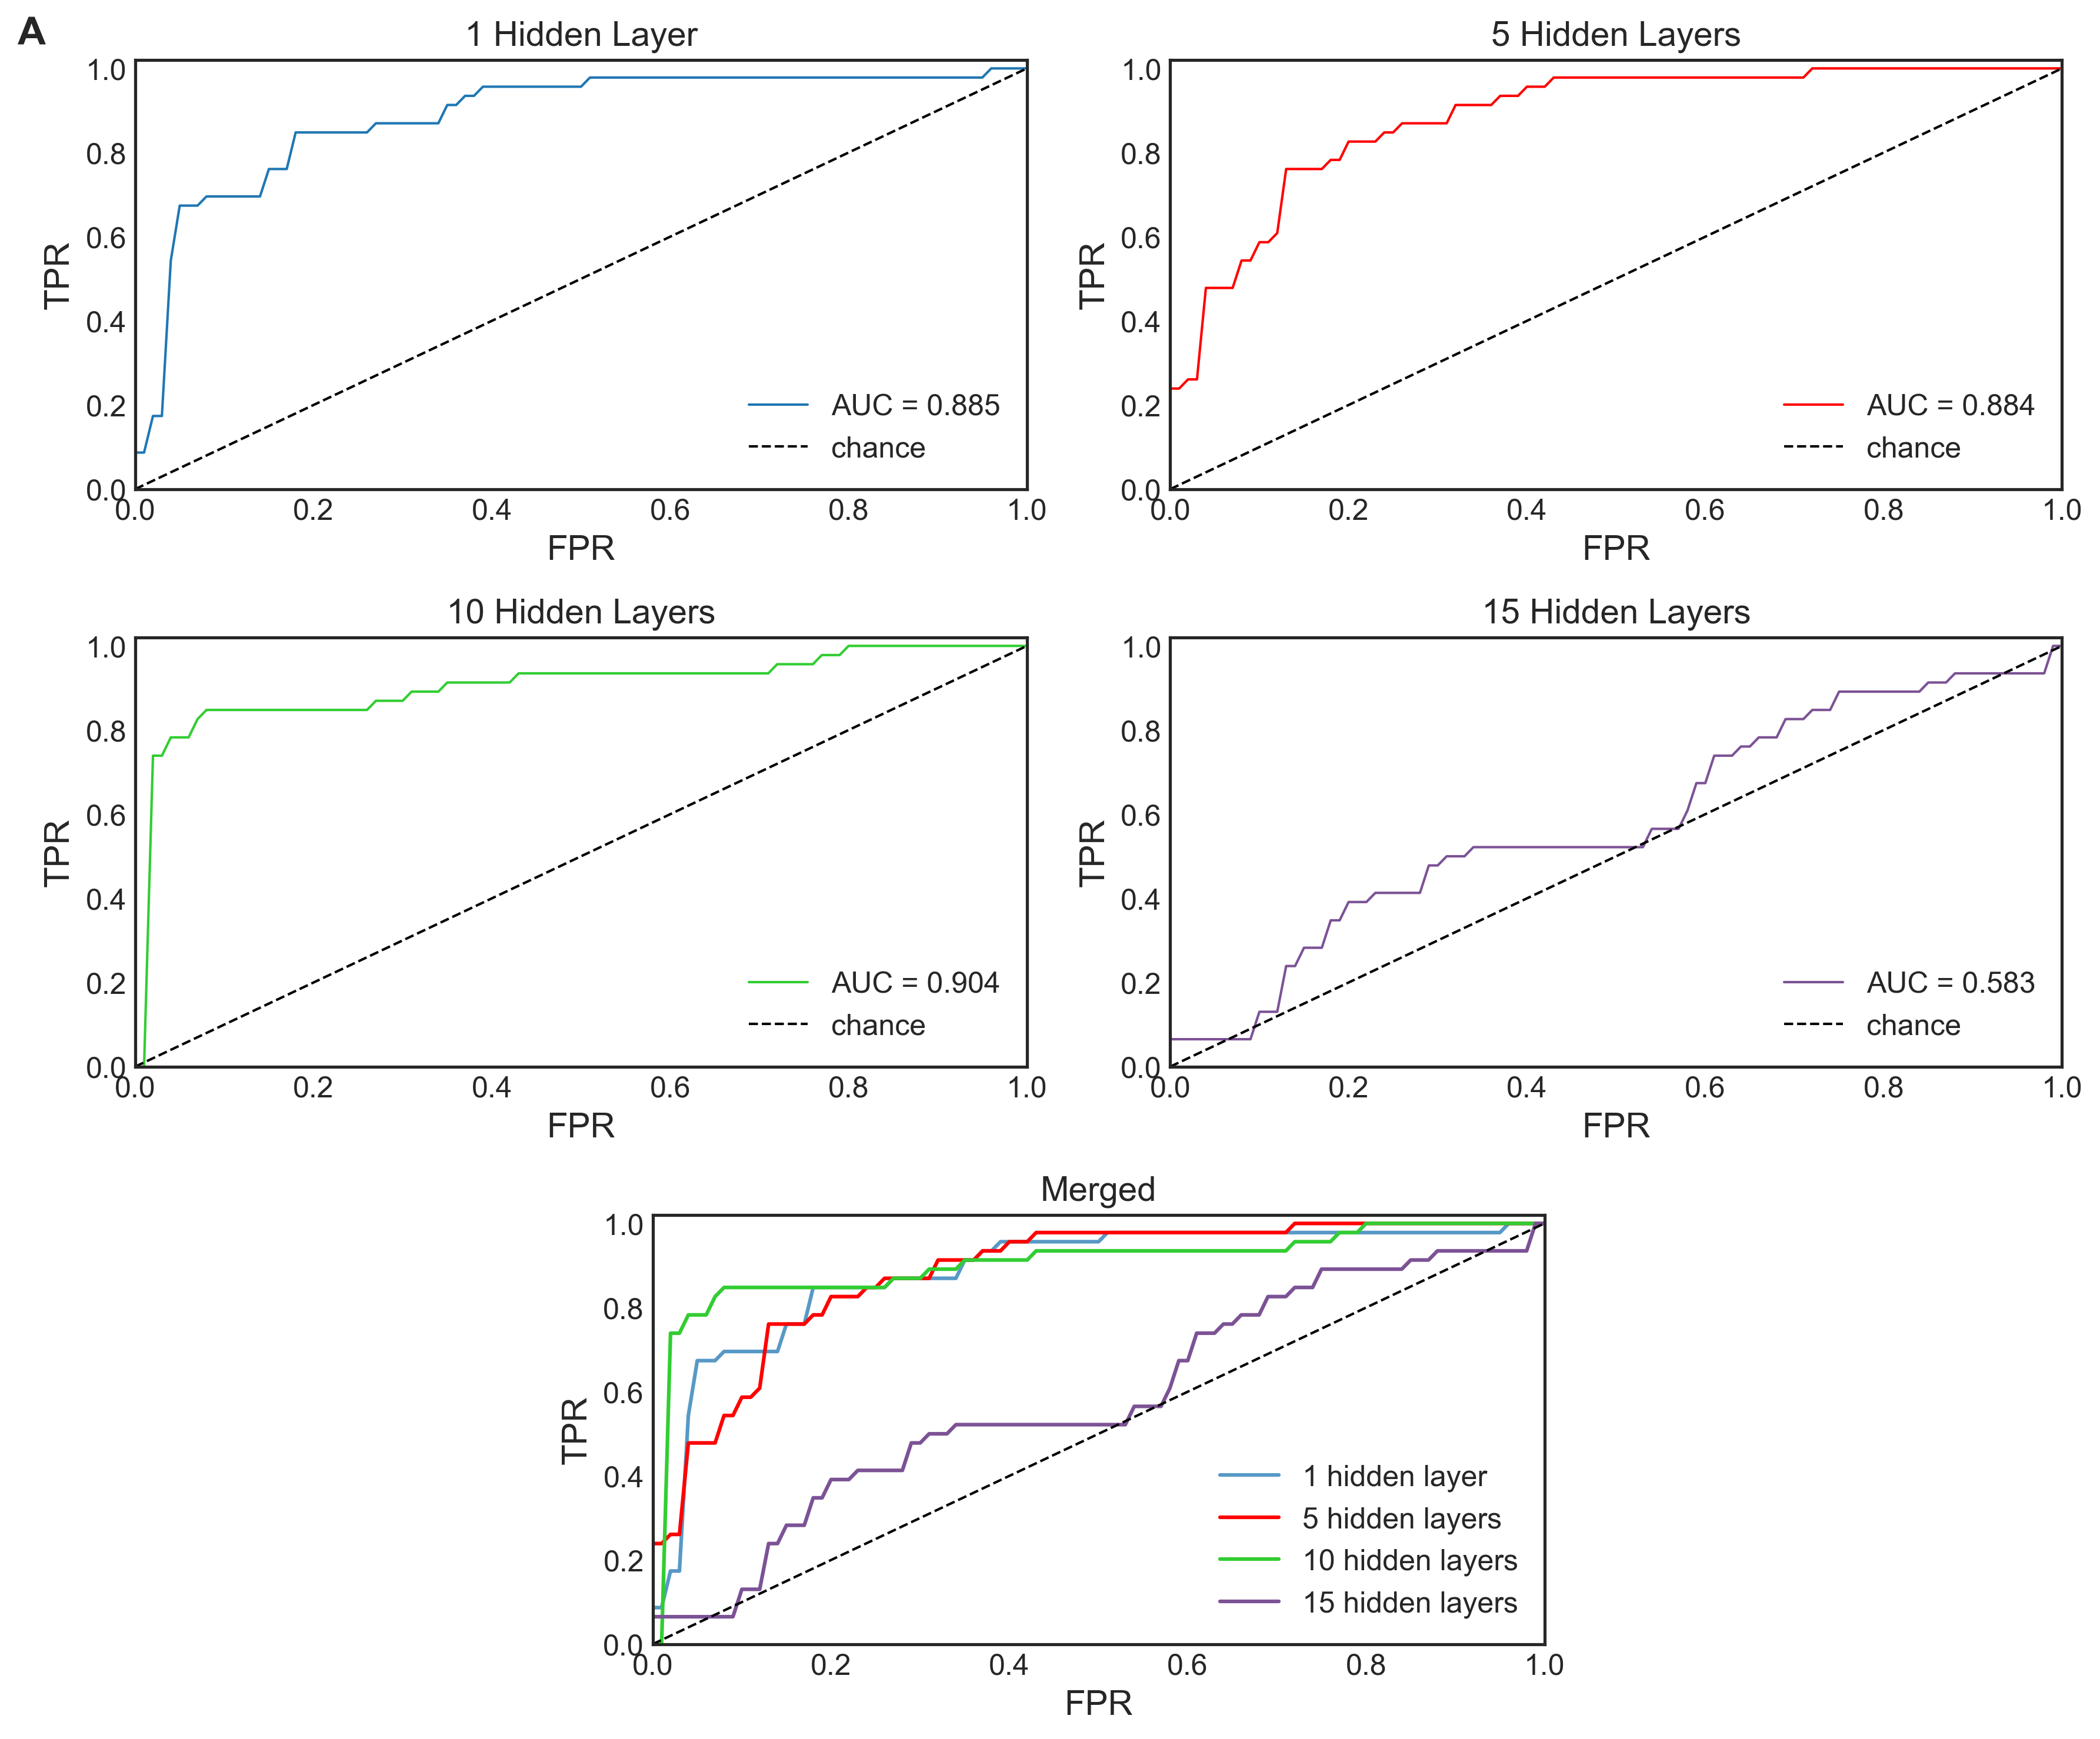
\includegraphics[width=\textwidth]{Figures/roc/final_roc.png}
	\end{subfigure}
	
	\begin{subfigure}[t]{\textwidth}
		\centering
		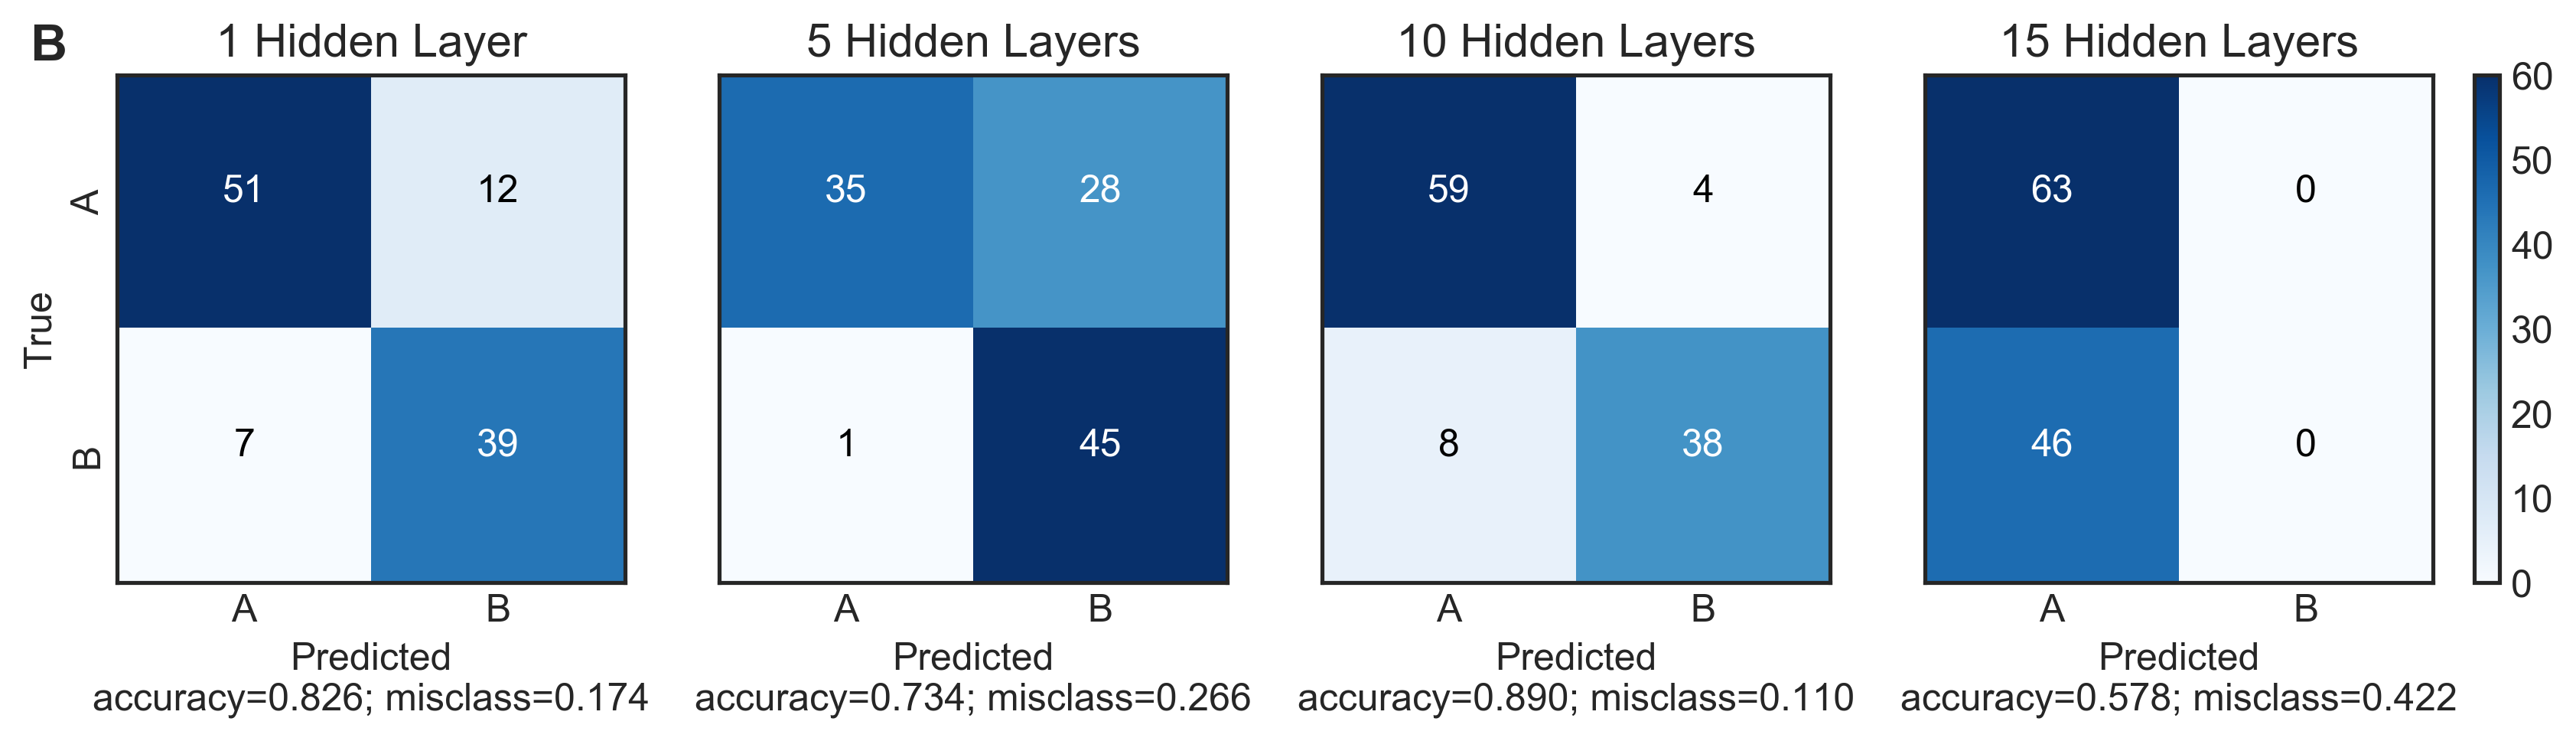
\includegraphics[width=\textwidth]{Figures/confusion_matrix/fcm_combined.png}
	\end{subfigure}
	
	\caption{(\textbf{A}) ROC curves for neural networks with 1, 5, 10, and 15 hidden layers on the testing dataset. (\textbf{B}) Confusion matrices for the 1, 5, 10, and 15 hidden layer neural network models on the testing set. The threshold for classification is determined using Youden's index from the training dataset (thresholds were 0.17, 0.10, 0.49, and 0.45 for neural networks with 1, 5, 10, and 15 hidden layers respectively). The models classify cell line microarray datasets into chemotherapy response cohorts A and B.}
	\label{fig:nnet}
\end{figure*}



Unsupervised learning via k-means clustering of the cancer cell line transcriptomes indicated substantially different responses to chemotherapies. Since k-means clustering instantiates randomly-placed centroids, we ran the algorithm several times, and each iteration returned similar results. Using these distinct therapy response cohorts, we developed a deep learning binary classifier to predict drug response groups based on transcriptomic data. We analyzed four neural network architectures: 1, 5, 10, and 15 hidden layers (Fig. \ref{fig:neural_vis}). Prior to model evaluation, SMOTE was used to prevent class imbalance in the training dataset; no synthetic samples were added to response group A and 146 synthetic samples were added to response group B (original data had 289 samples in response group A and 143 samples in response group B; 432 total original samples, 578 total samples with SMOTE). SMOTE was not applied to the testing dataset to ensure generalizability to real-world data. During training, hyperparameter optimization via grid search with 3-fold cross-validation returned similar results for each model: 50 epochs, batch size of 32, 50 neurons per hidden layer, L2 kernel regularization with $\lambda=10^{-3}$, Adam as the optimizer, and a normal kernel initializer. Following this, we validated the various architectures with 5-fold stratified cross-validation.

On the training data, the neural network with 5 hidden layers performed the best on the validation fold with 93.1\% accuracy (88.8\% for 1 hidden layer, 84.5\% for 10 hidden layers, 56.9\% for 15 hidden layers). The mean AUC across the 5 folds were $0.965 \pm 0.017$, $0.957 \pm 0.0144$, $0.913 \pm 0.026$, and $0.515 \pm 0.115$ for the neural networks with 1, 5, 10, and 15 hidden layers respectively (Fig. \ref{fig:nnet_train}). Here the relative ratio between the model’s false positive rate and its true positive rate was averaged between 5 stratified k-folds. The mean ROC curves plotted from the training set showed relatively small variance across all 5 k-folds, as evidenced by the small width of the confidence interval (Fig. \ref{fig:nnet_train}). The mean AUC for the 5 trials was used to compare the four network architectures. While there were no significant differences between AUC for the 1, 5, and 10 hidden layer models, the model with 15 hidden layers performed significantly worse compared to the rest. Youden's index was determined from the ROC curves, and the thresholds were 0.17, 0.10, 0.49, and 0.45 for neural networks with 1, 5, 10, and 15 hidden layers respectively. These thresholds were used to classify the cell lines into chemotherapeutic response groups in the final evaluation of neural network performance (i.e., on the testing dataset).

The testing dataset showed slightly different metrics to that from the training dataset (Fig. \ref{fig:nnet}). Similar to the training data, the neural network with 15 hidden layers performed the worst of the models evaluated. The neural network with 10 hidden layers performed the best on the testing dataset with an accuracy of 89.0\% (82.6\% for 1 hidden layer, 73.4\% for 5 hidden layers, and 57.8\% for 15 hidden layers). The AUC was 0.885, 0.884, 0.904, and 0.583 for the neural networks with 1, 5, 10, and 15 hidden layers respectively. Of note, the neural network with 15 hidden layers classified all cell lines into the responder group. The weighted F1 scores for the neural networks with 1, 5, 10, and 15 layers were 0.83, 0.73, 0.89, and 0.42 respectively.


% Discussion
\section{Discussion}
Differences in chemotherapeutic response between and within cancer types and clinical subgroups represents a critical challenge to current clinical management \cite{hetero, plasticity}. Heterogeneity in treatment response results in subsets of patients bearing significant side-effect burden with minimal treatment efficacy, substantially limiting quality of life and limiting future treatment course. Although there have been multiple attempts to identify molecular and clinical features predictive of response to targeted chemotherapies, there remains considerable variability within subgroups (ex: anatomical location of the tumour) identified using these factors. In this study, we accurately cluster cancer cell lines into defined groups based on response to a large range of chemotherapeutics and to create a deep learning transcriptomic model capable of accurately categorizing samples into these defined groups.

Using cell line chemotherapeutic efficacy obtained from the GDSC consortium, we employed unsupervised clustering techniques to identify two defined therapeutic response groups with significantly different responses to a multitude of standard chemotherapies. We demonstrate that commonly-used clinical criteria to predict chemotherapeutic performance -- such as anatomical location and morphologic subtype of cell lines, as well as TP53 and KRAS mutation status -- failed to identify defined clusters of cells with similar therapeutic responses (Fig. \ref{fig:overall_pca}). The consistent poor separability using these criteria and the relatively homogeneous distribution of cell responses to chemotherapeutics across major anatomical regions provide evidence for the utility of a pan-drug predictive biomarker. Given the separability and the large feature space of the microarray data, a neural network was developed to classify cell lines into therapeutic response groups. This model may inform clinicians and researchers of the predicted therapeutic response of their patients to various chemotherapies.

Following the determination of two defined chemotherapeutic groups based on the GDSC dataset, we used a biologically agnostic feature selection algorithm, Boruta, to reduce the original set of 16,382 genes to a subset of 300 genes and to limit preliminary bias due to multicollinearity in the neural network models. The genes were then fed into neural networks, which were optimized using a grid search (Table \ref{tab:params}). Each network was carefully monitored for overfitting during training (loss value on the validation set was observed to decrease during training across all models). To minimize overfitting, we applied L2 kernel regularization ($\lambda=10^{-3}$), batch normalization, and dropout layers with a 0.3 dropout rate to each hidden layer. To account for imbalanced classes during the cross-fold evaluations, we utilized SMOTE and stratified k-folds on the training dataset. The mean ROC curves plotted from the training set showed relatively small variance across all 5 k-folds, suggesting that the error from each model is relatively stable, and thus generalizable to real-world data.

Evaluation of the final neural network models on the testing dataset showed that the best network architecture utilized 10 hidden layers, demonstrating an 89.0\% accuracy in classifying cell lines into chemotherapeutic response groups (Fig. \ref{fig:nnet}). The efficacy of the network validates our postulate that gene expression is a prime determinant of chemotherapeutic response, and that cell lines of similar gene expression profile respond similarly to most chemotherapies.

The significantly lower accuracy of the neural network with 15 hidden layers on the testing data (57.8\%) as compared to the networks with 1, 5, and 10 hidden layers indicates severe overfitting. Overfitting was also evidenced by both the low AUC and high loss for this model during all stages of the neural network evaluation pipeline. The lower accuracy of the neural networks with 1 (82.6\%) and 5 hidden layers (73.4\%) compared to that with 10 hidden layers (89.0\%) suggests that therapeutic response cohorts cannot be separated by a linear classifier and that classical machine learning techniques are insufficient to capture the complexity of the dataset. To this end, a 10 hidden layer model is the ideal neural network depth to analyze the GDSC dataset.

The deep learning transcriptomic model consists of 300 gene inputs, and KEGG pathway enrichment analyses indicated that predictive genes are significantly associated with numerous pathways, most notably the PI3K signalling and focal adhesion pathways (Fig. \ref{fig:kegg}). Interestingly, there is a growing body of literature that suggests that PI3K/Akt pathway dysregulation may be associated with chemotherapeutic resistance in numerous different cancer and treatment contexts \cite{huang_2009}. Several studies have identified increases in Akt signalling in cancer cell lines exposed to chemotherapy and radiotherapy \cite{mapk, wort, phos}. Moreover, significant increases in Akt have been identified in chemoresistant and radioresistant cancer models \cite{cholangio}. Similarly, several studies have identified focal adhesion as a potential protective mechanism for various cancer cells. In fact, inhibition of particular integrin isoforms has been shown to increase the susceptibility of various cancer cell lines to conventional chemo/radiotherapies \cite{focal_adhesion}. Our results provide further evidence that dysregulation of PI3K signalling and focal adhesion may play a role in chemotherapy resistance in a pan-cancer context.

A major limitation of our study was the availability of large datasets to train our model. Here we faced a $p \gg n$ problem as machine learning models expect that the number of observations $n$ will be much larger than the number of features $p$. To minimize this bias, we applied the Boruta algorithm to reduce our 16,382 genes by 541 cell lines dataset to a 300 by 541 matrix. The algorithm has been shown in various studies to be an effective feature selection method in high dimensional omics datasets \cite{boruta}.

Future investigations will look to validate the predictive ability of the model to categorize chemotherapeutic response in various cancer types using the current transcriptomic signature. Further, we aim to recursively subcluster within the response groups to increase the resolution of classifications, providing clinicians and researchers with increasingly granular subsets of patients with sufficiently similar chemotherapeutic response patterns. It is likely that the model accuracy will vary between therapy targets, and as such, further studies can make use of our project pipeline to create a stratified model whereby the drug class and target are additional inputs. In addition, biochemical features of gene targets may provide additional insights, especially for the interpretability of the neural network output. It may also be interesting to select relevant genes using a different feature selector given that Boruta specifically operates on patterns of statistical relationships rather than biological relationships. As such, Boruta is sensitive to hyperparameter values. Our use of Boruta was primarily motivated by its efficacy demonstrated by prior studies of the algorithm as compared to other feature selectors \cite{boruta, deep_cell}. It is possible that a feature selection method informed by gene function and linkage disequilibrium could yield a different set of relevant genes.


% Conclusions
\section{Conclusions}
Using transcriptomic data from pan-cancer cell lines, two chemotherapeutic response clusters were identified via unsupervised learning in the form of k-means clustering. The Boruta feature selection algorithm was used to select a 300 gene subset that served as inputs to multiple neural networks. We determined that a network with 10 hidden layers was the most accurate model, producing a binary classifier to predict cell line therapy response with 89.0\% accuracy. To our knowledge, a pan-cancer, pan-drug chemotherapeutic classification model has not been investigated. Future studies will investigate the efficacy of our model to predict chemotherapy response in various cancer types and treatment contexts.


% Acknowledgements
\section*{Acknowledgements}
We wish to acknowledge the STEM Fellowship for organizing the 2020 Big Data Challenge, as well as Roche, SAS, Canadian Science Publishing, Digital Science, Altmetric, and Overleaf for their contributions that enabled this competition. We would like to thank our mentor, Dr. Daiva Nielsen for her feedback on our paper. We would also like to acknowledge Matthew Pietrosanu, Stephen Styles, Danyi Liu, and Boya Peng for their critical statistical review of the manuscript draft.


\bibliography{bibliography}

\clearpage

\onecolumn
\renewcommand{\thepage}{S\arabic{page}}
\renewcommand{\thesection}{S}
\renewcommand{\thetable}{S\arabic{table}}
\renewcommand{\thefigure}{S\arabic{figure}}
\setcounter{figure}{0}

\section{Supplementary Data}
\subsection{Figures}

% clustering figure
\begin{figure*}[!ht]
	\centering
	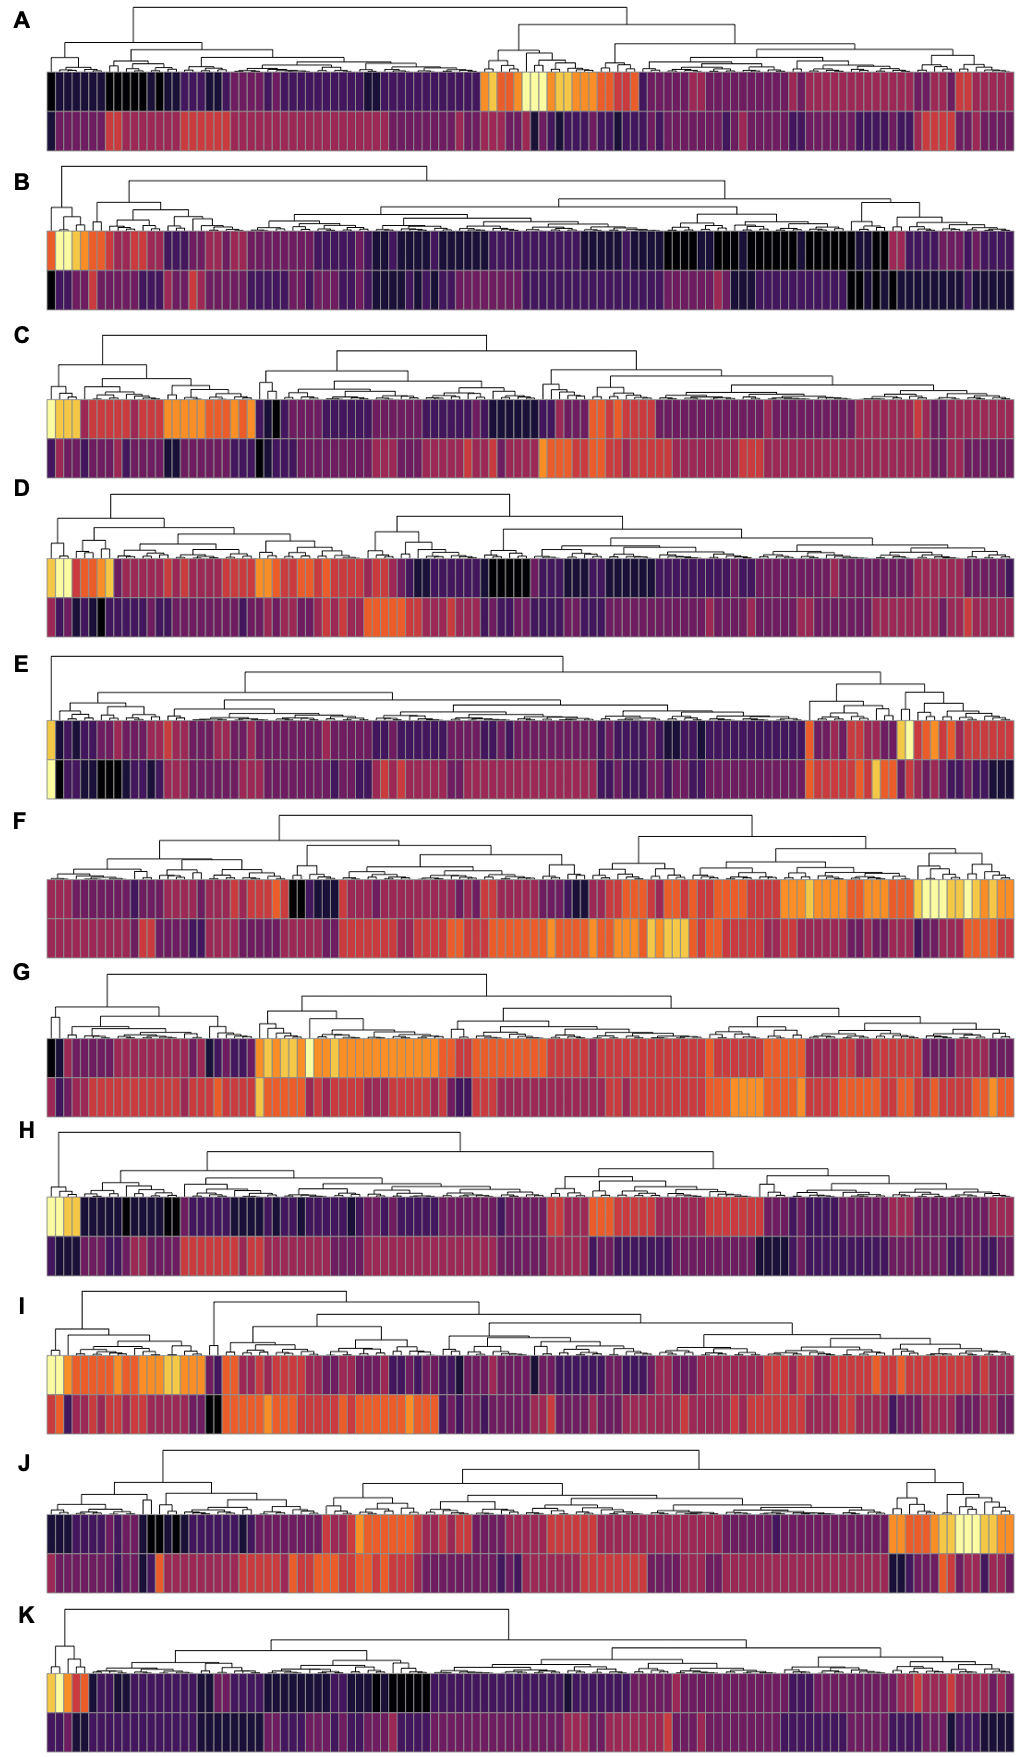
\includegraphics[height=0.8\textheight]{Figures/intra.png}

	\caption{Intra-cancer differences in chemotherapeutic efficacy between identified chemotherapeutic clusters. Clusters are arranged into cluster A (upper group) to cluster B (lower group) for each figure. The cancers represented are (\textbf{A}) non-small cell lung cancer, (\textbf{B}) breast cancer, (\textbf{C}) other digestive tract cancers, (\textbf{D}) small-cell lung cancer, (\textbf{E}) other nervous system cancers, (\textbf{F}) skin cancers, (\textbf{G}) urogenital cancers, (\textbf{H}) lymphomas, (\textbf{I}) colorectal cancers, (\textbf{J}) bone cancers, and (\textbf{K}) leukemia.}
	\label{fig:intra}
\end{figure*}

% neural network architecture figure
\begin{figure*}[ht]
    \centering
    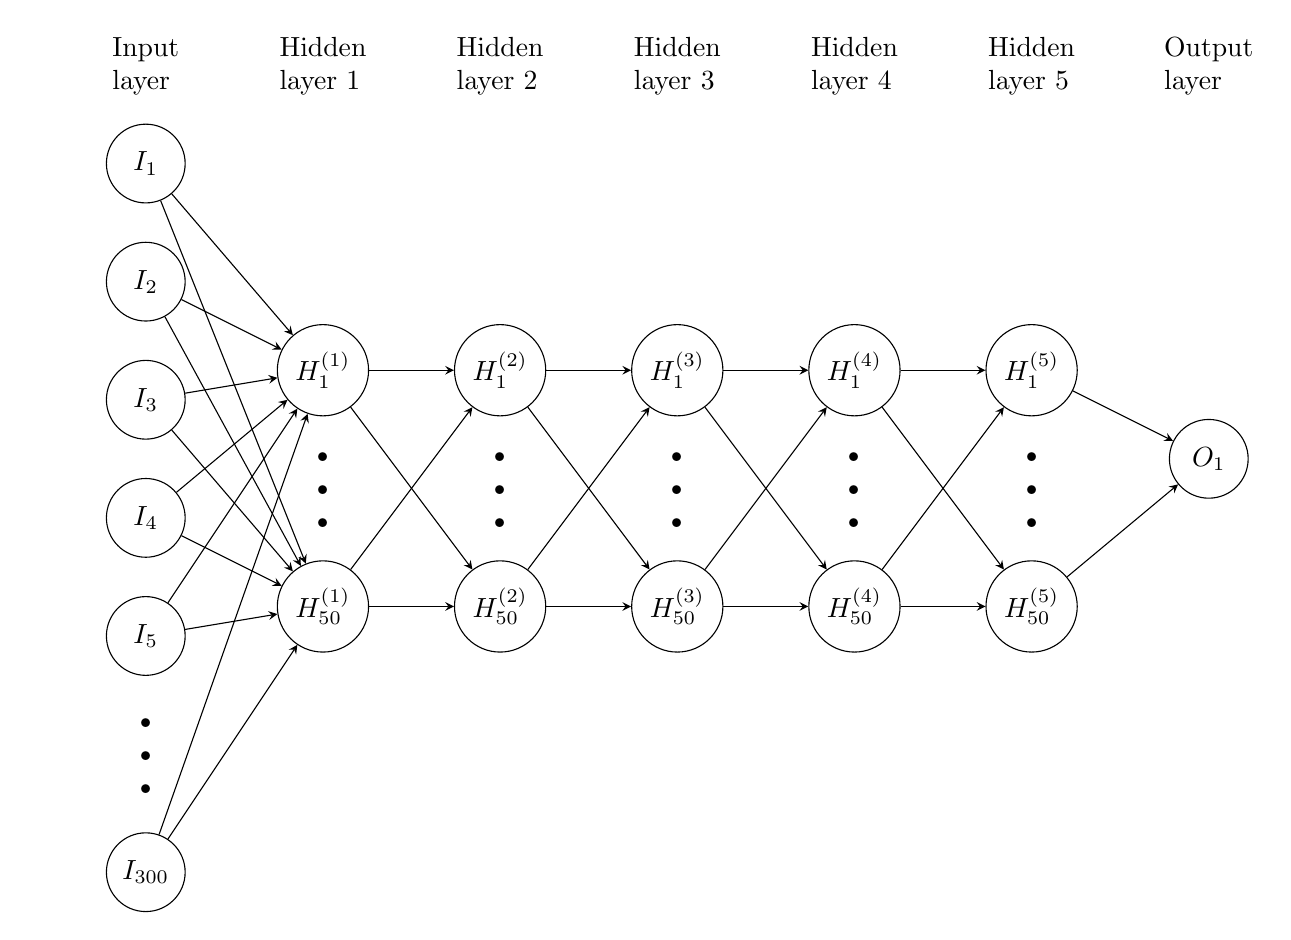
\begin{tikzpicture}[x=1.5cm, y=1.5cm, >=stealth]
    
        % nodes
        \foreach \m/\l [count=\y] in {1,2,3,4,5,missing,300}
            \node [every neuron/.try, neuron \m/.try] (input-\m) at (0,-\y) {\lmao{\l}};
        
        \foreach \m/\l [count=\y] in {1,missing,50}
            \node [every neuron/.try, neuron \m/.try] (hidden-\m) at (1.5,-1.75-\y) {\foo{\l}};

        \foreach \m/\l [count=\y] in {1,missing,50}
            \node [every neuron/.try, neuron \m/.try] (hidden1-\m) at (3,-1.75-\y) {\hehe{\l}};
    
        \foreach \m/\l [count=\y] in {1,missing,50}
            \node [every neuron/.try, neuron \m/.try] (hidden2-\m) at (4.5,-1.75-\y) {\hehetwo{\l}};
    
        \foreach \m/\l [count=\y] in {1,missing,50}
            \node [every neuron/.try, neuron \m/.try] (hidden3-\m) at (6,-1.75-\y) {\hehethree{\l}};
            	
        \foreach \m/\l [count=\y] in {1,missing,50}
			\node [every neuron/.try, neuron \m/.try] (hidden4-\m) at (7.5,-1.75-\y) {\hehefour{\l}};
    
        \foreach \m/\l [count=\y] in {1}
            \node [every neuron/.try, neuron \m/.try] (output-\m) at (9,0-2.5-\y) {$O_1$};

        % arrows
    
    	% input to hidden 1
        \foreach \l [count=\i] in {1,2,3,4,5,300}
            \foreach \k [count=\j] in {1,50}
              \draw [->] (input-\l) -- (hidden-\k);
   
    	% hidden 1 to hidden 2
        \foreach \l [count=\i] in {1,50}
            \foreach \k [count=\j] in {1,50}
              \draw [->] (hidden-\l) -- (hidden1-\k);
    
    	% hidden 2 to hidden 3
        \foreach \l [count=\i] in {1,50}
            \foreach \k [count=\j] in {1,50}
              \draw [->] (hidden1-\l) -- (hidden2-\k);
    
    	% hidden 3 to hidden 4
        \foreach \l [count=\i] in {1,50}
            \foreach \k [count=\j] in {1,50}
              \draw [->] (hidden2-\l) -- (hidden3-\k);
              
    	% hidden 4 to hidden 5
		\foreach \l [count=\i] in {1,50}
		\foreach \k [count=\j] in {1,50}
		\draw [->] (hidden3-\l) -- (hidden4-\k);
    
    	% hidden 5 to output
        \foreach \l [count=\i] in {1,50}
            \foreach \k [count=\j] in {1}
              \draw [->] (hidden4-\l) -- (output-\k);

        % labelling layers
        \foreach \l [count=\x from 0] in {Input\\layer, Hidden\\layer 1, Hidden\\layer 2, Hidden\\layer 3, Hidden\\layer 4, Hidden\\layer 5, Output\\layer}
            \node [align=left, above] at (\x*1.5, -0.5) {\l};

    \end{tikzpicture}
    \caption{Neural network architecture representation with 5 hidden layers (300 inputs). Inputs include the feature-selected genes from the cell line microarray dataset. Each hidden layer is batch-normalized with an L2 kernel regularization penalty ($\lambda=10^{-3}$) and a dropout rate of 0.3.}
    \label{fig:neural_vis}
\end{figure*}


% neural net evaluation figure
\begin{figure*}[!ht]
	\centering
		\begin{subfigure}[t]{\textwidth}
			\centering
			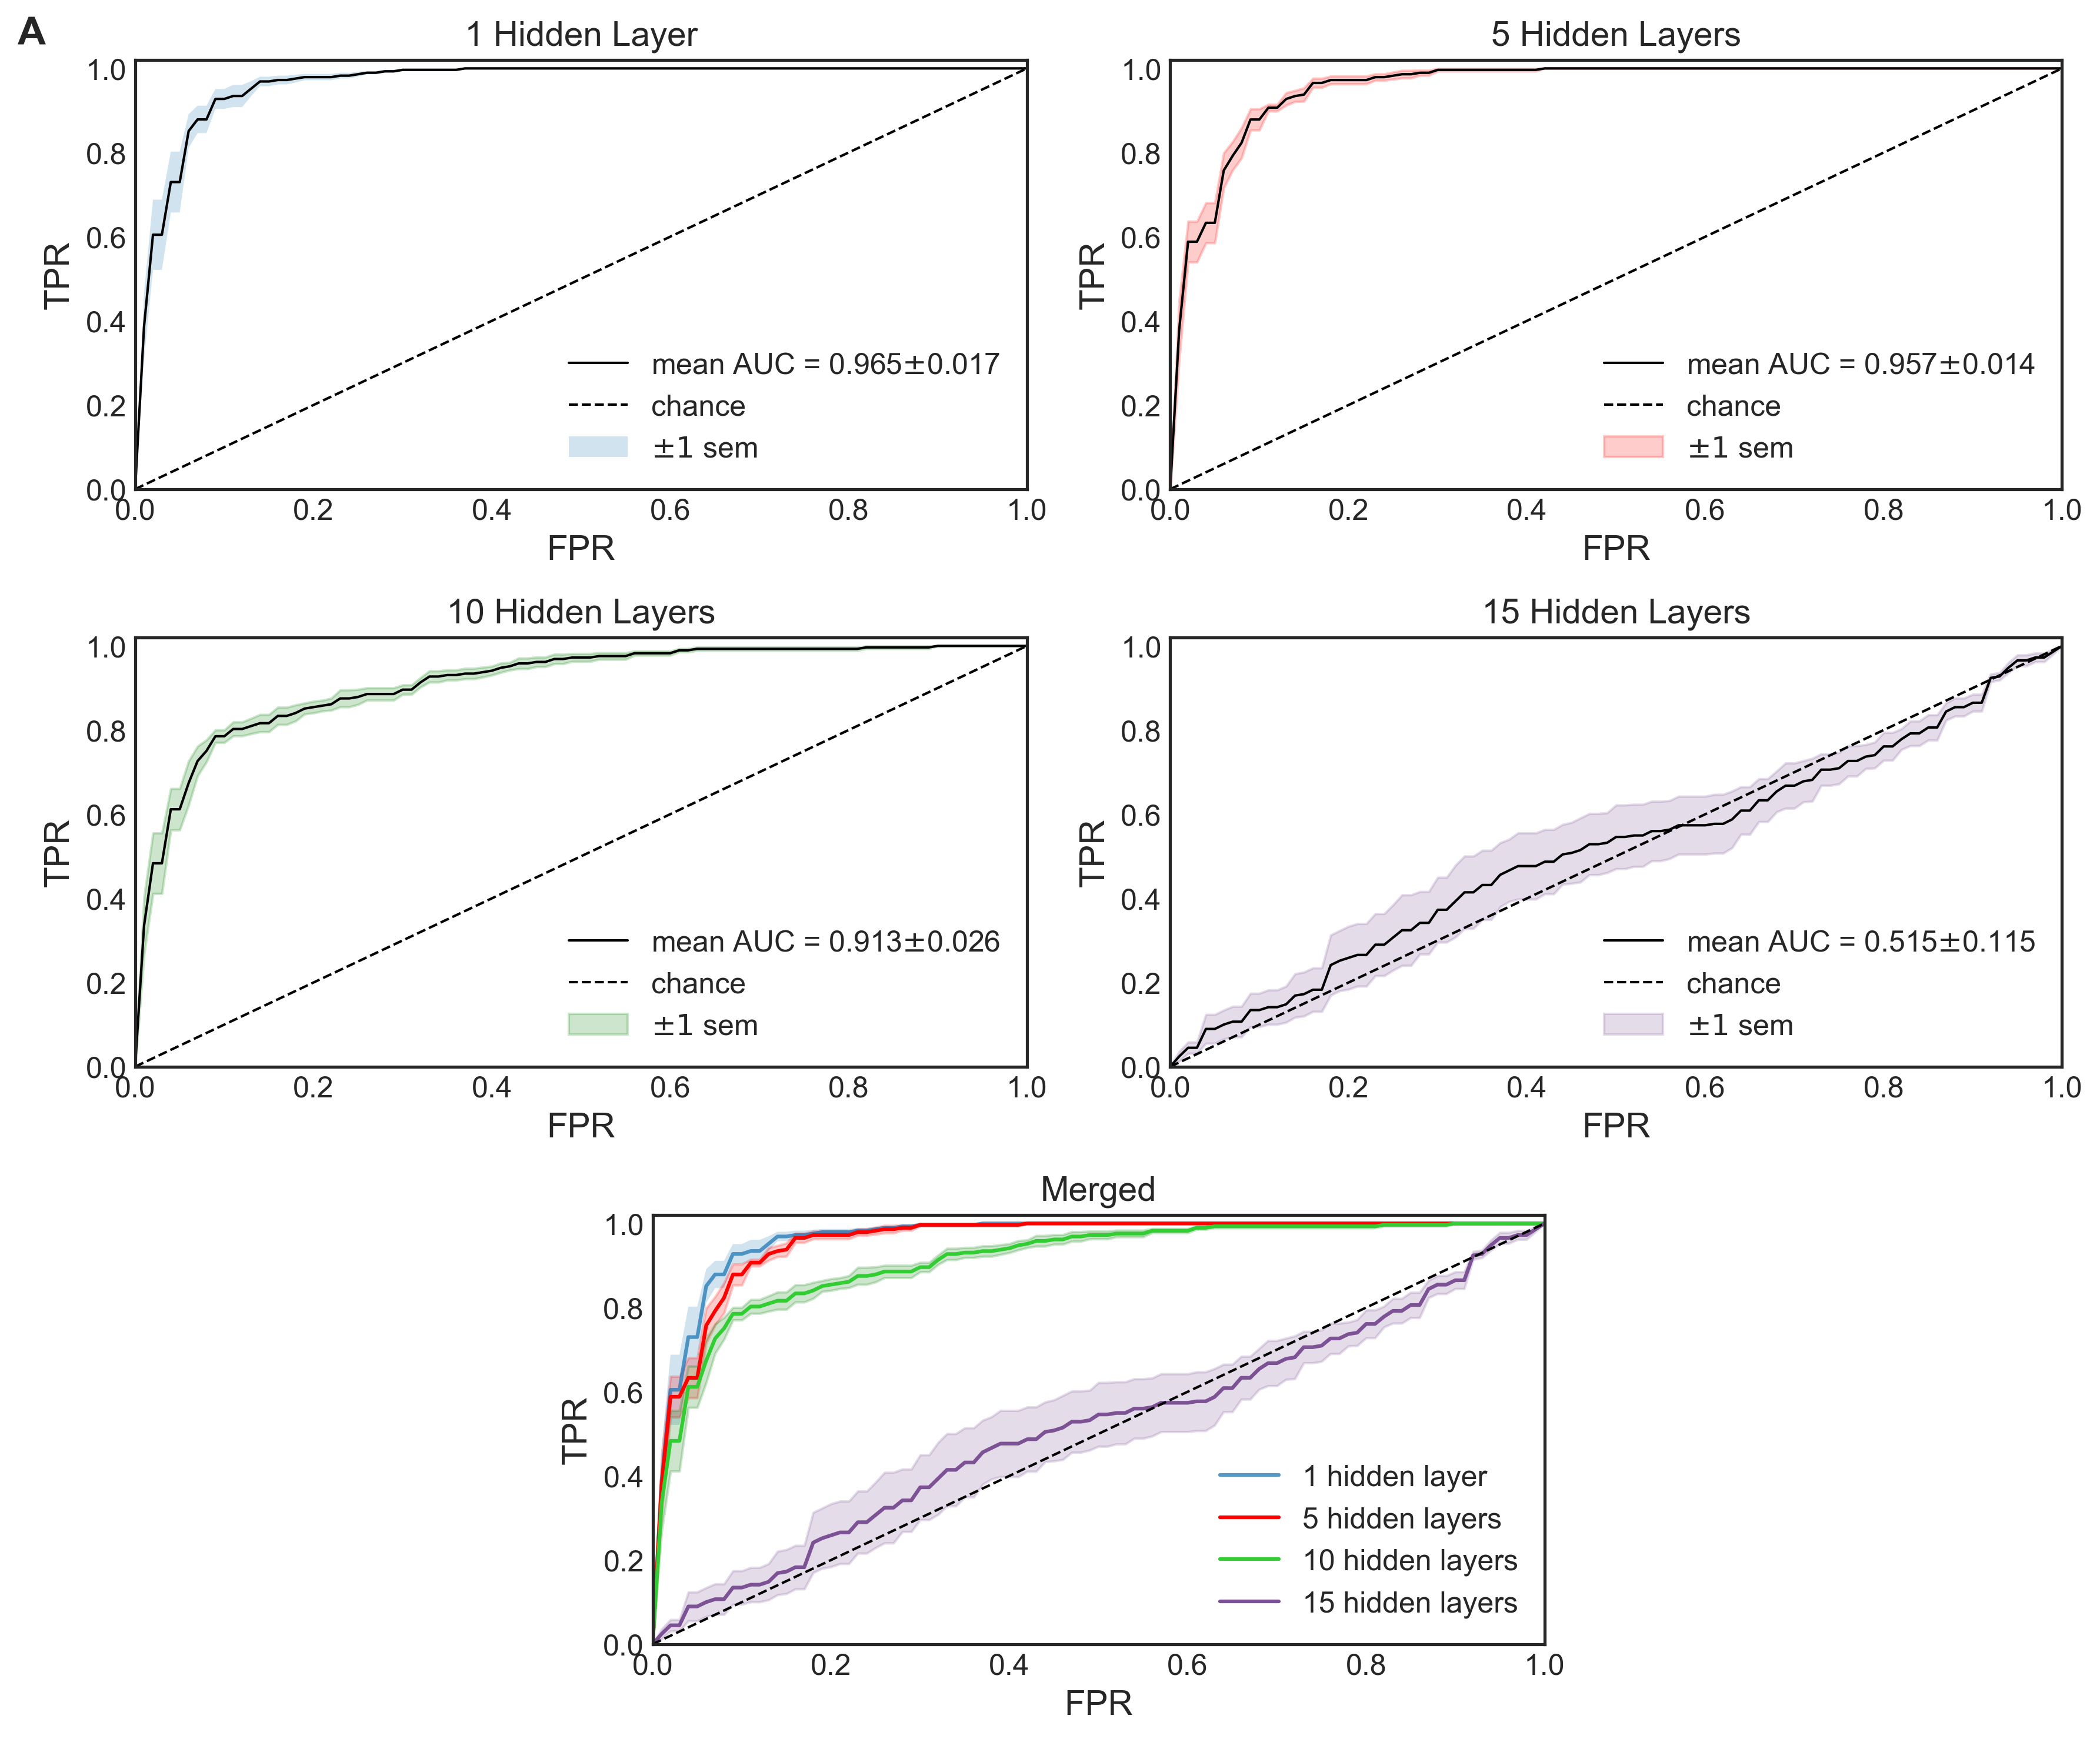
\includegraphics[width=\textwidth]{Figures/roc/cv_roc.png}
		\end{subfigure}

	\begin{subfigure}[t]{\textwidth}
		\centering
		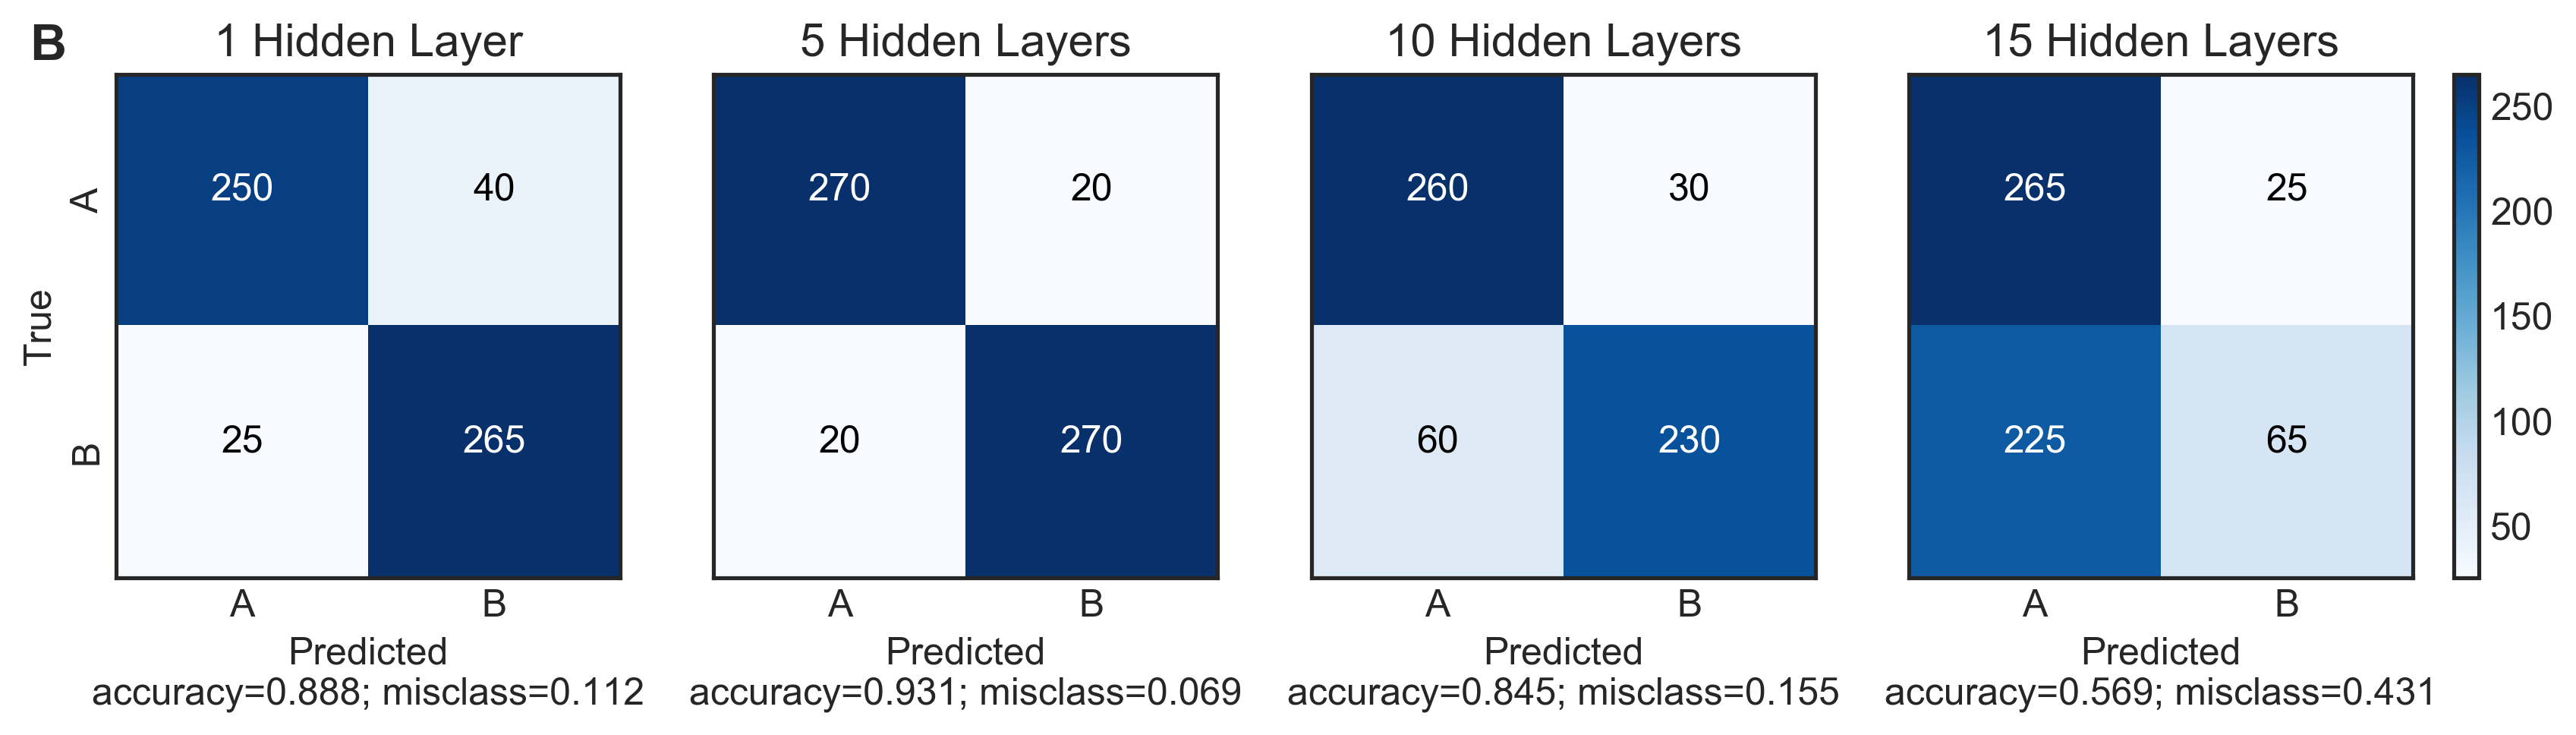
\includegraphics[width=\textwidth]{Figures/confusion_matrix/cm_combined.png}
	\end{subfigure}
	
	\caption{(\textbf{A}) ROC curves for 1, 5, 10, and 15 hidden layers neural network models with confidence bands of $\pm 1$ standard error of the mean (sem). Each model was subject to 5-fold stratified cross-validation on the training set and the mean ROC curve for the validation set across all trials was plotted. The threshold corresponding to Youden's index was used to classify cell lines into response groups for the testing data (thresholds were 0.17, 0.10, 0.49, and 0.45 for neural networks with 1, 5, 10, and 15 hidden layers respectively; corresponding Youden's indices reported in Table \ref{tab:params}). (\textbf{B}) Confusion matrices for the 1, 5, 10, and 15 hidden layer neural network models on the validation set. The models classify cell line microarray datasets into chemotherapy response cohorts. The threshold to classify cell lines into response cohorts is 0.5.}
	\label{fig:nnet_train}
\end{figure*}

\clearpage

\subsection{Tables}
% parameters
\begin{table*}[h]
    \caption{Grid search parameters to optimize all implemented neural network architectures (1, 5, 10, and 15 hidden layers). Each grid search underwent 3-fold cross-validation on the training data. Optimal parameters: 50 epochs, batch size of 32, 50 neurons, $\lambda=10^{-3}$, Adam as optimizer, normal kernel initializer.}
    \centering
    \label{tab:params}
    \begin{tabular}{c c c c l l}
        \toprule
        Epochs & Batches & Neurons & $\lambda$ (L2 reg) & Optimizer & Kernel initializer \\
        \midrule
        25 & 16 & 50 & 1e-4 & Sgd & Normal \\
        50 & 32 & 100 & 1e-3 & Adagrad & Uniform \\
        75 & 64 & 150 & 1e-2 & Adam & Glorot uniform \\
        \bottomrule
    \end{tabular}
\end{table*}


% Results
\begin{table*}[h]
	\caption{Classification scores for the 1, 5, 10, and 15 neural networks on the testing data.}
	\centering
	\label{tab:class_scores}
	\begin{tabular}{l c c c c}
		\toprule
		Hidden layers & Accuracy & AUC & Weighted F1 score & Youden's index\\
		\midrule
		1 & 82.6\% & 0.885 & 0.83 & 0.736 \\
		5 & 73.4\% & 0.885 & 0.73 & 0.690 \\
		10 & 89.0\% & 0.904 & 0.89 & 0.780 \\
		15 & 57.8\% & 0.583 & 0.42 & 0.500 \\
		\bottomrule
	\end{tabular}
\end{table*}


\end{document}















